\documentclass[prd,
               reprint,
               aps,
               preprintnumbers,
               nofootinbib,
               longbibliography,
               floatfix]{revtex4-2}

\usepackage{amsmath}
\usepackage{amssymb}
\usepackage{graphicx}
\usepackage{dcolumn}
\usepackage{bm}
\usepackage{hyperref}

\begin{document}

% -------------------------------------------------------------
% \textcolor{blue}{===========================================}
% -------------------------------------------------------------
\title{IR Matching of the Cosmological Constant in a Classical
Vacuum-Response EFT}

\author{Robinson Bueno Parra}
\email{robinbuenoparra8@gmail.com}
\affiliation{Independent Researcher, Spain}
\affiliation{GitHub Repository: \url{https://github.com/robinson388/constante-cosmologica}}
\affiliation{Zenodo Digital Repository DOI: \href{https://doi.org/10.5281/zenodo.21540551}{10.5281/zenodo.21540551}}

\date{\today}

\begin{abstract}
We present a self-contained, covariant classical effective field 
theory of an emergent vacuum response field $P_{\text{vac}}$ that 
unifies gravitational, astrophysical, and quantum phenomena across 
all physical scales without ab initio fine-tuning. By decoupling 
the macroscopic response substrate from renormalized quantum vacuum 
energy, the framework introduces a non-local spatial memory kernel 
and fluid-relaxation dynamics into the space-time fabric. At 
cosmological scales, a constitutive infrared matching condition at 
the horizon scale yields a parameter-free entropy attractor 
fraction ($x_\star \simeq 0.689$) matching Planck satellite data 
within a $+0.17\%$ margin of error. At galactic and stellar scales, 
the framework successfully reproduces the asymptotically flat 
rotation curves of the SPARC database without dark matter halos and 
tracks General Relativity orbits around Sgr A* within a 
$\delta\theta \approx 0.101\text{ mas}$ limit. In the microscopic 
quantum regime, formulating the electron as a continuous vacuum 
pressure distribution yields the exact Bohr radius and ground-state 
energy of the Hydrogen atom. Furthermore, we extend this framework 
to high-energy regimes, reframing multi-TeV resonances at CERN 
as short-range solitonic vacuum excitons, predicting a distinct 
mass differential of $\Delta M = +0.007\text{ GeV}$ validated 
against CMS-like datasets, thereby providing distinct, falsifiable 
targets across vastly separated frontiers.
\end{abstract}



\maketitle

%%%%%%%%%%%%%%%%%%%%%%%%%%%%%%%%%%%%%%%%%%%%%%%%%%%%%%%%%%%%%%%%%%%%%%%%%%%%%%%%%%%%%%%%%
% \textcolor{blue}{====================================================================}
% \textcolor{blue}{SECTION I: INTRODUCTION}
% \textcolor{blue}{====================================================================}
%%%%%%%%%%%%%%%%%%%%%%%%%%%%%%%%%%%%%%%%%%%%%%%%%%%%%%%%%%%%%%%%%%%%%%%%%%%%%%%%%%%%%%%%%

\section{Introduction}

The cosmological constant problem remains arguably the most profound
crisis in modern theoretical physics~\cite{Weinberg1989,Polchinski2006,
Martin2012}. Within the standard framework of Quantum Field Theory
(QFT), the vacuum energy density is computed as the sum of zero-point
energies across all fields up to a fundamental cutoff scale. If the
Planck mass ($M_{\text{Pl}}$) is adopted as the natural ultraviolet
(UV) limit, the theoretical vacuum energy density scales as
$\rho_{\text{th}} \sim M_{\text{Pl}}^4 \sim 10^{92}\text{ kg/m}^3$.
Conversely, cosmological measurements from the cosmic microwave
background (CMB) and distant Type Ia Supernovae place the observed
dark energy density at $\rho_{\text{obs}} \sim 10^{-26}\text{ kg/m}^3$
~\cite{Planck2020,Riess1998,Perlmutter1999}. This yields an
unprecedented mismatch of approximately 120 orders of magnitude,
frequently referred to as the cosmological constant
catastrophe~\cite{Carroll2001}.

To reconcile this immense fine-tuning dilemma, standard $\Lambda$CDM
cosmology treats $\Lambda$ either as an ad-hoc geometric integration
constant or introduces dynamical scalar fields (e.g., quintessence)
that require delicate, unnatural potentials~\cite{Zlatev1999,
Peebles1988,Wetterich1988,Caldwell1998}. Alternative approaches
attempt to exploit holographic bounds or modified gravity
schemes~\cite{Padmanabhan2003,tHooft1993,Susskind1995,Bousso2002,
Cohen1999,Li2004,Clifton2012,Sotiriou2010,DGP2000}, yet a direct
analytical bridge linking microscopic vacuum parameters to macroscopic
cosmic parameters without fine-tuning has remained elusive.

In this work we separate three layers that prior drafts conflated:
\begin{enumerate}
\item a covariant \emph{classical} EFT for $P_{\rm vac}$
(Eq.~\eqref{eq:master_action});
\item a \emph{constitutive} IR matching $\Omega_{\rm bd}=a_0/(cH_0)$
(Sec.~\ref{sec:constitutive_closure}), numerically the same content
as the long-standing MOND--$H_0$ coincidence~\cite{Milgrom1983,
Famaey2012};
\item a passive $\Lambda$CDM background $\Omega_\Lambda$ fixed by
CMB input, not output from $a_0$.
\end{enumerate}

The title phrase ``vacuum'' refers to the classical response field
$P_{\rm vac}$, not to a renormalized QFT vacuum energy.
Inspired by the thermodynamic reading of horizons~\cite{Jacobson1995},
we treat $R_H=c/H_0$ as an IR matching scale, not a material shell
(Sec.~\ref{sec:horizon_reframe}).

To address the galactic rotation curve anomaly without invoking ad-hoc,
undetected dark matter particles, we propose that the physical vacuum
is not a passive geometric background. Instead, it behaves as an active
structured medium endowed with non-local memory and a plastic-like
rheological response. Under the action of compact baryonic sources and
localized core vorticity, the vacuum field undergoes a dynamical stress
redistribution. This mechanism generates an extended effective mass
profile that naturally accounts for asymptotically flat galactic
rotation curves.

\subsection{Observables, benchmarks, and falsifiable targets}
\label{sec:observables_prd}

To meet standard \emph{Physical Review D} expectations on testability, we
state explicitly which published data anchor the parameters and which
outputs are falsifiable predictions versus consistency checks.

To establish the empirical validity of our classical EFT framework,
we define three independent observational benchmarks. First, the
spatial variation of the response field $P_{\rm vac}$ modifies the
local geodesic equation, introducing a non-local acceleration
correction. This modification must systematically reproduce the flat
rotation curves of the SPARC database without inflating the stellar
mass-to-light ratios.

The primary numerical benchmark is the localized memory length scale,
empirically constrained to $r_m \approx 6.6\text{ kpc}$ for Milky
Way-like systems. This scale serves as a fixed parameter that breaks
the typical halo-mass degeneracy inherent to standard dark matter
parametrizations like the Navarro-Frenk-White (NFW) profile.

Furthermore, the model provides distinct, falsifiable targets at
astrophysical and cosmological scales:
\begin{itemize}
\item \textbf{Edge velocity scale invariance:} At extreme radii, the
induced velocity asymptotically approaches a common scale
$v_{\rm mem, edge} \sim 100 \pm 20\text{ km/s}$, decoupled from the
total baryonic mass.
\item \textbf{Lensing-rotation consistency:} The effective surface
density $\Sigma(R)$ derived from stress redistribution must predict
gravitational lensing deflection profiles that match kinematic data
without secondary modifications.
\item \textbf{Environmental modulation:} As a non-local rheological
response, the value of $r_m$ is predicted to vary weakly under the
influence of external tidal fields or group-scale membership.
\end{itemize}

\paragraph{Fixed observational anchors (inputs).}
Background cosmology uses Planck 2018 values
$H_0=67.4\,\mathrm{km\,s^{-1}\,Mpc^{-1}}$, $\Omega_\Lambda=0.688$,
and $\Omega_m=0.315$~\cite{Planck2020}. Recent DESI baryon-acoustic-%
isochronous (BAO) constraints and the classic SDSS acoustic peak%
~\cite{DESI2024,Eisenstein2005} are compatible with this passive
$w=-1$ anchor at percent-level precision in $(\Omega_m h^2,\,H_0)$;
they are cited as external checks, not refit inputs to the Planck
anchors listed here. The galactic scale is
$a_0=1.20\times10^{-10}\,\mathrm{m/s^2}$ (SPARC/MOND phenomenology)%
~\cite{Milgrom1983,Famaey2012,Sanders2002}. Local gravity
uses post-Newtonian parameters $\gamma=\beta=1$ at the field minimum,
consistent with Cassini $\gamma-1=(2.1\pm2.3)\times10^{-5}$%
~\cite{Will2014,Bertotti2003}. Tensor propagation uses $v_{\rm gw}=c$,
compatible with GW170817--GRB~170817A~\cite{Abbott2017GW}.

\paragraph{Internal consistency benchmarks (not new discoveries).}
Table~\ref{tab:validation} and Sec.~\ref{sec:test_scope} compare the
EFT to Mercury perihelion, SPARC-type rotation speeds, Sirius~B
redshift, core saturation, and binary GW speed at the level of
order-of-magnitude agreement with standard benchmarks.

\paragraph{Falsifiable targets specific to this framework.}
(i)~Horizon attractor fraction $x_\star=\Omega_m/(2\alpha_s)$ from
$H_0$, $P_0$, and Gibbons--Hawking entropy \emph{without}
$\Omega_\Lambda$ in the $\chi$ sector (Sec.~\ref{sec:horizon_attractor};
current post-diction $x_\star\simeq 0.689$ vs.\ Planck $0.688$).
(ii)~Failure of volumetric three-dimensional hysteresis as a
$\Lambda$ estimator (null test; Sec.~\ref{app:3d_null}).
(iii)~Sensitivity of $x_\star$ to the cubic entropy slope
$\zeta/\chi$ (Table~\ref{tab:overfit_audit}).
(iv)~Galactic rotation from the integrated AQUAL limit of the scalar
gradient law (script \texttt{test2\_sparc\_field.py}).
A failure of any of (i)--(iii) at the quoted percent level would refute
the constitutive closure as implemented; (iv) is an open numerical
channel.



\section{Dynamical Vacuum and Non-Local Memory Transport}
\label{sec:dynamical_vacuum}

\subsection{Conservation and Relaxation Dynamics}
We model the physical vacuum as a coherent emergent substrate governed by
a scalar density field $\rho(\mathbf{x}, t)$. The temporal evolution of
the pressure and density states within this medium is dictated by a
modified continuity equation incorporating diffusion and linear local
relaxation:

\begin{equation}
\frac{\partial \rho}{\partial t} = -\nabla \cdot (\rho \mathbf{v}) +
D\nabla^2 \rho - \gamma(\rho - \rho_0)
\end{equation}

where $\rho_0$ represents the background vacuum density at fundamental
equilibrium, $D$ is the effective diffusion coefficient, and $\gamma$
denotes the relaxation rate. The term $-\gamma(\rho - \rho_0)$ provides
the physical restoring force of the vacuum as it attempts to recover its
equilibrium state after being compressed by baryonic structures. The
velocity field $\mathbf{v}$ driving the phase transport is given by:

\begin{equation}
\mathbf{v} = \mathbf{v}_{\text{source}} +
\mathbf{v}_{\text{vortex}} - \lambda \nabla \rho
\end{equation}

where $\mathbf{v}_{\text{source}}$ accounts for external driving forces,
$\mathbf{v}_{\text{vortex}}$ couples the flow to intrinsic angular
momentum (core vorticity and spin), and $-\lambda \nabla \rho$ is the
non-linear response to localized vacuum pressure gradients.

\subsection{Rheological Memory Kernel and Gravitational Modification}
To capture the persistent plastic-like behavior of the vacuum under
gravitational deformation, the accumulated stress $\sigma(r)$ is not
dissipated locally. Instead, it undergoes a non-local redistribution
mediated by a spatial memory operator:

\begin{equation}
\mathcal{M}[\sigma](r) = \int_{0}^{r} K(r, r') \sigma(r') \, dr'
\end{equation}

where the finite-range exponential kernel is parameterized as:

\begin{equation}
K(r, r') \sim \exp\left( -\frac{|r - r'|}{r_m} \right)
\end{equation}

Here, $r_m$ defines the characteristic spatial memory scale of the
effective substrate. This rheological modification transforms the
acceleration profile, mapping the non-local phase redistribution into a
stable gravitational velocity support:

\begin{equation}
v_{\text{obs}}^2(r) = v_{\text{bar}}^2(r) + v_{\text{mem}}^2(r)
\end{equation}

where $v_{\text{bar}}(r)$ is the standard Newtonian baryonic velocity,
and $v_{\text{mem}}^2(r) = M_{\text{eff}}(r)/r$ provides the continuous
structural support required to sustain flat profiles without unseen
matter.


% -------------------------------------------------------------
% \textcolor{blue}{===========================================}
% -------------------------------------------------------------
\subsection{Vacuum Energy-Momentum Tensor}

We consider an effective stress-energy tensor for the vacuum 
given by:
\begin{equation}
\label{eq:Tvac}
T_{\mu\nu}^{\text{vac}} = -\rho_{\text{vac}} c^2 g_{\mu\nu},
\end{equation}
where $\rho_{\text{vac}}$ represents the coherent vacuum energy 
density. The Einstein field equations assume the standard 
form:
\begin{equation}
\label{eq:einstein_split}
G_{\mu\nu} = \frac{8\pi G}{c^4} \left( T_{\mu\nu}^{\text{matter}} 
+ T_{\mu\nu}^{\text{vac}} \right).
\end{equation}

By defining the effective cosmological constant as 
$\Lambda = \frac{8\pi G}{c^2} \rho_{\text{vac}}$, the 
unified field equation reduces naturally to:
\begin{equation}
\label{eq:einstein_lambda}
G_{\mu\nu} + \Lambda g_{\mu\nu} = \frac{8\pi G}{c^4} 
T_{\mu\nu}^{\text{matter}}.
\end{equation}

% -------------------------------------------------------------
\subsection{Lorentz Invariance and Energy-Momentum Conservation}
\label{sec:conservation}

The vacuum sector is encoded by a \emph{Lorentz scalar} energy density
$\rho_{\Lambda}$ at the passive minimum $P_{\rm vac}=P_0$ (fixed by the
cromatic2/Planck $\Lambda$CDM background), while the dynamical boundary
piece $\rho_{\rm bd}$ of Eq.~\eqref{eq:rho_boundary} is tied to the
galactic threshold $a_0$.
Both are Lorentz scalars.
Under a local Lorentz transformation
$L^\alpha{}_\mu$, scalars and tensors transform as
$\rho_{\Lambda}\to\rho_{\Lambda}$ and
$T^{\text{vac}}_{\mu\nu}\to L^\alpha{}_\mu L^\beta{}_\nu
T^{\text{vac}}_{\alpha\beta}$, so Eq.~\eqref{eq:Tvac} defines a covariant,
Lorentz-invariant stress-energy tensor of the form expected for a
spatially homogeneous vacuum with equation of state $w=-1$.

The total stress-energy is
\begin{equation}
\label{eq:Ttotal}
T_{\mu\nu}^{\text{tot}}
=
T_{\mu\nu}^{\text{matter}}
+
T_{\mu\nu}^{\text{vac}}
=
T_{\mu\nu}^{\text{matter}}
-\rho_{\text{vac}} c^2 g_{\mu\nu}.
\end{equation}
The effective action (minimal coupling, constant $\rho_{\text{vac}}$) is
\begin{equation}
\label{eq:effective_action_constant}
\begin{aligned}
S = &\frac{c^4}{16\pi G} \int\! d^4x \sqrt{-g}\, R \\
&- \int\! d^4x \sqrt{-g}\, \rho_{\text{vac}} c^2 
+ S_{\text{matter}}[g_{\mu\nu}, \psi].
\end{aligned}
\end{equation}


Variation with respect to $g^{\mu\nu}$ reproduces
Eqs.~\eqref{eq:einstein_split}--\eqref{eq:einstein_lambda} with
$\Lambda=\frac{8\pi G}{c^2}\rho_{\text{vac}}$.
Because $\rho_{\text{vac}}$ is \emph{not} promoted to a dynamical field,
no extra propagating degree of freedom is introduced beyond standard
General Relativity (GR) plus matter.

The contracted Bianchi identity,
\begin{equation}
\label{eq:bianchi}
\nabla_\mu G^{\mu\nu}=0,
\end{equation}
together with Eq.~\eqref{eq:einstein_lambda}, implies matter conservation in the usual GR sense:
\begin{equation}
\label{eq:matter_conservation}
\boxed{
\nabla_\mu T^{\mu\nu}_{\text{matter}}=0.
}
\end{equation}
Equation~\eqref{eq:matter_conservation} is the standard continuity law
for baryons, radiation, and other minimally coupled fluids; the vacuum
piece does not source an anomalous Lorentz-violating current because it
is absorbed into the geometric $\Lambda g_{\mu\nu}$ term.
Equivalently, using Eq.~\eqref{eq:Ttotal} and metric compatibility
($\nabla_\mu g^{\mu\nu}=0$),
\begin{equation}
\label{eq:Ttot_conservation}
\nabla_\mu T^{\mu\nu}_{\text{tot}}
=
\nabla_\mu T^{\mu\nu}_{\text{matter}}=0,
\end{equation}
the same total-divergence closure as in $\Lambda$CDM with constant
$\Lambda$.

\paragraph{Relation to General Relativity.}
In the weak-field, slow-motion limit ($\Phi/c^2\ll 1$,
$|\mathbf{v}|\ll c$), Eq.~\eqref{eq:einstein_lambda} reduces to the Newtonian Poisson equation
with an effective source
$\rho_{\text{eff}}=\rho_{\text{matter}}+\rho_{\text{vac}}$ and no
preferred frame beyond the metric itself. Solar-system and binary-pulsar
constraints are therefore inherited from the same minimal-coupling
structure as GR, provided local corrections from $a_0$ remain
subdominant at laboratory and planetary scales (benchmark Test~1 in
Table~\ref{tab:validation}). The present framework is thus not a
replacement of the Einstein equations but a \emph{boundary-fixed}
identification $\rho_{\Lambda}=\Omega_\Lambda\rho_{\rm crit}$ with dynamical
coupling $\Omega_{\rm bd}=a_0/(cH_0)$ addresses the IR magnitude of the
120-order hierarchy without breaking Lorentz symmetry or matter
conservation (Sec.~\ref{sec:scope_lambda}).

% -------------------------------------------------------------
\section{Covariant Field Theory (Self-Contained Core)}
\label{sec:master}

To avoid external manuscript dependence, the essential dynamics are
recorded here.

\paragraph{Metric signature.}
Throughout Sec.~\ref{sec:master} we use the mostly-plus convention
$(-,+,+,+)$, so that for a static weak field $g_{00}\simeq-(1+2\Phi/c^2)$
and $g_{ij}\simeq(1-2\Phi/c^2)\delta_{ij}$. With this signature, the
scalar kinetic energy density is $T_P^{00}\supset+\frac12(\partial_t
P_{\rm vac})^2$ and the action term $-\frac12 g^{\mu\nu}\nabla_\mu
P\nabla_\nu P$ is positive-definite (no phantom branch). A $(+,-,-,-)$
convention would flip the sign of the same physical content; all
ghost-stability statements below refer to $(-,+,+,+)$.

The fundamental action of our effective field theory framework is 
formulated as follows:

% =====================================================================
% ACTION FORMULATION
% =====================================================================
\begin{equation}
\label{eq:master_action}
\begin{aligned}
\mathcal{S} = \int\! d^4x\sqrt{-g}\, \Big[ &\frac{c^4}{16\pi G}R \\
&-\frac12 g^{\mu\nu}\nabla_\mu P_{\rm vac}\nabla_\nu P_{\rm vac} \\
&-V(P_{\rm vac}) + \mathcal{L}_{\rm matter}(\psi,\tilde{g}_{\mu\nu}) \\
&-\frac14 B(P_{\rm vac})F_{\mu\nu}F^{\mu\nu} \\
&-\frac14 C(P_{\rm vac})F_{\mu\nu}\tilde{F}^{\mu\nu} \Big],
\end{aligned}
\end{equation}
% =====================================================================

where the matter fields are coupled to the physical Jordan-frame metric 
defined conformally as $\tilde{g}_{\mu\nu} = A^2(P_{\rm vac})g_{\mu\nu}$. 
The exponential coupling function $A(P_{\rm vac})$ takes the form:

% =====================================================================
% CONFORMAL COUPLING FUNCTION
% =====================================================================
\begin{equation}
\label{eq:A_quadratic}
A(P_{\rm vac}) = \exp\left[ -\frac{\lambda_v}{2c^2}
(P_{\rm vac} - P_0)^2 \right].
\end{equation}
% =====================================================================

By differentiating this coupling relation with respect to the scalar 
response field, we obtain its corresponding field derivative:

% =====================================================================
% COUPLING DERIVATIVE
% =====================================================================
\begin{equation}
\alpha_A(P_{\rm vac}) = \frac{d\ln A}{dP_{\rm vac}} =
-\frac{\lambda_v}{c^2}(P_{\rm vac} - P_0).
\end{equation}
% =====================================================================

The macroscopically emergent screening mechanism is stabilized by a 
quartic self-interacting potential, which is explicitly defined as:

% =====================================================================
% STABILIZING POTENTIAL
% =====================================================================
\begin{equation}
\label{eq:Vquartic}
V(P_{\rm vac})=\frac{\lambda_P}{4}\left(P_{\rm vac}^2-P_0^2\right)^2,
\qquad \lambda_P>0.
\end{equation}
% =====================================================================

Taking the variation of the action with respect to the metric yields 
the modified gravitational field equations presented in 
Eq.~\eqref{eq:einstein_split}, where the vacuum stress-energy tensor 
$T_{\mu\nu}^{\rm vac}$ is evaluated at the $P_0$ field minimum. 
Concurrently, variation with respect to the scalar field yields the 
master wave equation:

% =====================================================================
% SCALAR MASTER FIELD EQUATION
% =====================================================================
\begin{equation}
\label{eq:box_pvac}
\Box P_{\rm vac}-\frac{dV}{dP_{\rm vac}} = -4\pi G\lambda_v T_{\rm eff},
\end{equation}
% =====================================================================

where $\Box \equiv g^{\mu\nu}\nabla_\mu\nabla_\nu$ represents the 
covariant d'Alembertian operator. The effective matter source term 
governing the right-hand side is structurally fixed by varying the 
matter Lagrangian $\mathcal{L}_{\rm matter}(\psi, \tilde{g}_{\mu\nu})$:

% =====================================================================
% EFFECTIVE SOURCE DEFINITION
% =====================================================================
\begin{equation}
\label{eq:Teff_def}
T_{\rm eff} \equiv \alpha_A(P_{\rm vac})\,T, \qquad T \equiv
g^{\mu\nu}T_{\mu\nu}^{\rm matter},
\end{equation}
% =====================================================================

where $T_{\mu\nu}^{\rm matter}$ denotes the standard matter tensor. 
For a perfect non-relativistic baryonic fluid operating under the chosen 
$(-,+,+,+)$ metric signature, the trace reduces as follows:

% =====================================================================
% NON-RELATIVISTIC MATTER TRACE
% =====================================================================
\begin{equation}
\label{eq:trace_nr}
T = g^{00}T_{00} + g^{ii}T_{ii} = -\rho_m c^2 + 3P \simeq -\rho_m c^2.
\end{equation}
% =====================================================================

To evaluate the mechanical stability of local overdensities, we expand 
the effective source to first order in the field excursion 
$\delta P \equiv P_{\rm vac}-P_0$. Substituting Eq.~\eqref{eq:A_quadratic} 
and Eq.~\eqref{eq:trace_nr} into the definition yields:

% =====================================================================
% LINEARIZED EFFECTIVE SOURCE
% =====================================================================
\begin{equation}
\label{eq:Teff_linear}
T_{\rm eff}^{(1)} = -\frac{\lambda_v}{c^2}\,\delta P\,T \simeq
+\frac{\lambda_v}{c^2}\,\delta P\,\rho_m c^2.
\end{equation}
% =====================================================================

Consequently, the core coupling product $\lambda_v T_{\rm eff}$ on the 
right-hand side of the scalar field equation Eq.~\eqref{eq:box_pvac} 
exhibits a definite and stable physical sign. A positive local density 
excess ($\rho_m>0$) matching a positive local displacement $\delta P>0$ 
sources the scalar equation attractively back toward the fundamental 
vacuum minimum. This mathematical setup entirely eliminates signs 
ambiguities within the linearized Poisson regime. Finally, at the flat 
cosmological background where $P_{\rm vac}=P_0$, the couplings yield 
$\alpha_A(P_0)=0$ and $T_{\rm eff}=0$, forcing linear tensor 
perturbations to propagate exactly at the speed of light $v_{\rm gw}=c$.



\subsection{Conformal Coupling, WEP, and Local Stability}
\label{sec:conformal_wep}

Matter propagates on $\tilde g_{\mu\nu}=A^2 g_{\mu\nu}$, i.e.\ a
Jordan-frame (matter-coupled) scalar--tensor structure of
Damour--Esposito-Far\`ese type~\cite{Damour1992,EspositoFarese2004,Will2014,Damour2010}.
Unlike $f(R)$ metric gravity~\cite{Sotiriou2010} or brane-world DGP
models~\cite{DGP2000}, the Einstein--Hilbert sector is standard and the
passive $\Lambda$ piece of Eq.~\eqref{eq:Tvac} is held fixed
(Sec.~\ref{sec:scope_lambda}).
Diffeomorphism invariance of $\mathcal{L}_{\rm matter}(\psi,\tilde g)$
implies that $T_m^{\mu\nu}$ is conserved with respect to $\tilde g$,
while the Einstein-frame current
\begin{equation}
\label{eq:exchange}
\nabla_\mu T_m^{\mu\nu}
=
Q^\nu,
\qquad
Q^\nu
=
\alpha_A(P_{\rm vac})\,T_m\,\nabla^\nu P_{\rm vac},
\end{equation}
vanishes \emph{linearly} at the minimum because $\alpha_A(P_0)=0$.
The Weak Equivalence Principle is therefore satisfied at $\mathcal{O}(\delta P)$
in the Solar System: there is no composition-dependent fifth force at
leading order; Jordan-frame deviations enter at $\mathcal{O}(\delta P^2)$.

\paragraph{Linear perturbations and chameleon screening.}
Write $P_{\rm vac}=P_0+\delta P$ with $|\delta P|\ll P_0$.
From Eq.~\eqref{eq:Vquartic},
\begin{equation}
\label{eq:mP}
m_P^2
\equiv
\left.\frac{d^2V}{dP_{\rm vac}^2}\right|_{P_0}
=
2\lambda_P P_0^2
>0,
\end{equation}
so the minimum is locally stable.
The linearized static limit of Eq.~\eqref{eq:box_pvac} is a screened
Yukawa equation for $\delta P$,
\begin{equation}
\label{eq:yukawa}
\left(\nabla^2-m_P^2\right)\delta P
=
-4\pi G\lambda_v\,T_{\rm eff}^{(1)},
\end{equation}
with Compton length $\lambda_C=\hbar/(m_P c)$.
In high-density environments (Solar System, $T\simeq -\rho_m c^2$),
the field is pinned to $P_0$ when $\lambda_C\ll R_{\rm env}$ (chameleon /
thin-shell limit)~\cite{Khoury2004,Hinterbichler2011}: the restoring term $m_P^2\delta P$ dominates any
residual drive from $\lambda_v T_{\rm eff}^{(1)}$, keeping
$|\delta P/P_0|\ll 1$
and preserving $\gamma=\beta=1$ at the level tested by Mercury
(Test~1)~\cite{Will2014}.
Operationally, $\lambda_P$ and $P_0$ must be chosen so that
$m_P R_\odot\gg 1$ locally while the IR matching of
Sec.~\ref{sec:covariant_hydro} still holds cosmologically; this is a
\emph{consistency constraint}, not an extra fit parameter in the
$\Lambda$ closure.

\paragraph{PPN emergence at the minimum.}
With Eqs.~\eqref{eq:A_quadratic}--\eqref{eq:mP},
\begin{equation}
\label{eq:ppn}
\gamma-1
=
-\frac{2\alpha_A^2}{1+\alpha_A^2}\Big|_{P_0}
=0,
\qquad
\beta-1
=
\frac{\alpha_A^2\beta_A}{2(1+\alpha_A^2)^2}\Big|_{P_0}
=0,
\end{equation}
with $\beta_A=d\alpha_A/dP_{\rm vac}=-\lambda_v/c^2$.
Thus GR is recovered at $P_0$ by construction of $A(P)$, and local
matter density does not ``drag'' the field off the minimum at linear order.

\paragraph{Identification of $a_0$ in the field theory.}
In the static weak-field limit,
$\mathbf{g}_{\rm eff}=-K_g\nabla P_{\rm vac}$ with exterior
$P_{\rm vac}=P_0-C/r$.
Saturation of the vacuum response defines
\begin{equation}
\label{eq:a0_field}
g_{\rm eff}(r_\ast)=a_0
\quad\Longleftrightarrow\quad
K_g C=r_\ast^2 a_0,
\end{equation}
linking $a_0$ to the dynamical field $P_{\rm vac}$, not to a bare
postulate.
The EM saturation scale $\beta_0=\alpha_{\rm EM}^{1/3}$ enters the
companion chromatic sector~\cite{cromatic2zenodo}; here only $K_g$ and
$P_0$ are required for the $\Lambda$ closure.

\paragraph{Homogeneous cosmological background (FLRW).}
On a spatially flat FLRW line element
$ds^2=-c^2dt^2+a^2(t)\,d\mathbf{x}^2$,
the background is \emph{homogeneous}:
$P_{\rm vac}=P_0$ and $\rho_{\rm vac}=\rho_\Lambda$ constant.
The radial profile $P_{\rm vac}=P_0-C/r$ (Sec.~\ref{sec:local_exterior}) applies
only on scales $r\ll R_H=c/H_0$ around bound systems (stars, halos).
On cosmological backgrounds $P_{\rm vac}=P_0$ exactly; linear CMB
isotropy is not sourced by a Hubble-scale $1/r$ gradient
(Sec.~\ref{sec:scale_separation}).

% -------------------------------------------------------------
\section{Boundary Matching and IR Closure}
\label{sec:cromatic2_bridge}

The effective medium is single-valued: one covariant $P_{\rm vac}$
with three empirically orthogonal readouts~\cite{cromatic2zenodo,gravedad3zenodo}:
\begin{enumerate}
\item \textbf{Electromagnetic (cromatic2).}
Chromatic transfer $\mathcal{G}(\lambda)=1-\exp[-A(\lambda/\lambda_0)]$
and host activation ${\cal S}_{\rm env}(\rho_m,|\nabla\Phi|,\ldots)$
imprint $H_0^{\rm obs}(\lambda,\beta_{\rm env})$ on SN/ladder versus
CMB anchors without relocating the sound horizon.
\item \textbf{Tensor (GRAVEDAD3).}
Parity-odd GW birefringence maps to an effective $(m_g,\lambda_g)$
bookkeeping channel; $v_{\rm gw}=c$ at linear order (Test~5).
\item \textbf{Background (this note).}
Passive stress~\eqref{eq:Tvac} with
$\nabla_\mu T^{\mu\nu}_{\rm matter}=0$
(Sec.~\ref{sec:conservation}) and the constitutive IR matching of
Sec.~\ref{sec:constitutive_closure} record the $\Lambda$ scale from
$(a_0,H_0)$.
\end{enumerate}
Local PPN parameters remain $\gamma=\beta=1$ at $P_{\rm vac}=P_0$
in the shared action~\cite{gravedad3zenodo}, so Solar-system
constraints (Test~1) and cromatic2's explicit no-PPN-modification
statement are aligned.
Figure~\ref{fig:rotation} and Test~2 use the \emph{phenomenological}
deep-MOND interpolation $g_{\rm eff}=\sqrt{g_{\rm N}a_0}$ as a
benchmark (not derived from Eq.~\eqref{eq:box_pvac} in this note).
The companion cromatic2 sector uses the same
$\beta_0=\alpha_{\rm EM}^{1/3}$ threshold in
$\phi_c(R)=\beta_0/\sqrt{R}$~\cite{cromatic2zenodo}.

\subsection{Horizon as IR Matching Surface, Not a Material Shell}
\label{sec:horizon_reframe}

The Hubble length $R_H=c/H_0$ is a \emph{coarse-grained infrared (IR) scale}
of the causal patch, analogous to the Rindler or cosmological horizon in
Jacobson's thermodynamic derivation~\cite{Jacobson1995,Gibbons1977,Bekenstein1973,Hawking1975}.
It is \emph{not} modelled as a spherical material wall centred on the
observer, nor as a unique geometric locus carrying mechanical pressure in
the literal fluid sense.
The ``boundary pressure'' language is shorthand for a \emph{matching
condition} between (i)~the passive FLRW background with density
$\rho_\Lambda$ and (ii)~the dynamical response saturation scale $a_0$
extracted from Eq.~\eqref{eq:a0_field}.
Different comoving observers on a homogeneous FLRW spacetime assign the
same $H_0$ and the same $\rho_{\rm crit}$; the matching is a property of
the EFT, not of a privileged spatial centre.

\subsection{Covariant Balance on an Expanding Background}
\label{sec:covariant_hydro}

Static Newtonian hydrostatics is \emph{not} obtained by sending
$H_0\to 0$ with $R_H=c/H_0\to\infty$ (which would erase the finite
matching scale).
Instead, one uses the \emph{quasi-static sub-horizon regime} at fixed
finite $H_0$: on scales $r\lesssim R_H=c/H_0$ and time scales
$t\lesssim H_0^{-1}$, comoving gradients of $P_{\rm vac}$ dominate over
$\partial_t^2 P_{\rm vac}$ when $|\delta P/P_0|\sim\mathcal{O}(1)$.
The primary covariant constraint is Eq.~\eqref{eq:ir_matching}; no
radial profile is evaluated at $r=R_H$.
On a flat FLRW background
$H=\dot a/a$, the comoving passive stress obeys
\begin{equation}
\label{eq:flrw_conservation}
\dot\rho_{\rm vac}+3H(\rho_{\rm vac}+P_{\rm vac}/c^2)=0,
\end{equation}
which is identically satisfied for $w=-1$.
The dynamical constraint enters through the Friedmann equation
\begin{equation}
\label{eq:friedmann}
H^2=\frac{8\pi G}{3}\left(\rho_m+\rho_{\rm vac}\right),
\end{equation}
on a spatially flat background~\cite{Peebles1993,Planck2020},
and the saturation matching
\begin{equation}
\label{eq:ir_matching}
a_0 \;\sim\; cH
\quad\Longleftrightarrow\quad
\Omega_{\rm bd}=\frac{a_0}{cH_0},
\end{equation}
where the $\sim$ denotes the IR identification of the field-theoretic
scale Eq.~\eqref{eq:a0_field} with the Hubble flow of the \emph{same}
homogeneous patch.
Equation~\eqref{eq:ir_matching} is the IR statement; it is not obtained
by extrapolating $P_{\rm vac}=P_0-C/r$ to $r=R_H$
(Sec.~\ref{sec:scale_separation}).

\subsection{What Is and Is Not Solved for \texorpdfstring{$\Lambda$}{Lambda}}
\label{sec:scope_lambda}

\textbf{Solved (UV--IR hierarchy):} why the observed vacuum energy density
is $\sim10^{-27}\,\mathrm{kg/m^3}$ rather than $\sim10^{92}\,\mathrm{kg/m^3}$
when a UV cutoff is misapplied---Eq.~\eqref{eq:rho_boundary} ties the IR
scale to $(a_0,H_0)$ without $M_{\rm Pl}^4$ summation.

\textbf{Not solved (absolute $\Omega_\Lambda$):} the dominant passive fraction
$\Omega_\Lambda\simeq 0.69$ is still fixed by CMB/$\Lambda$CDM compatibility
(as in the cromatic2 early-universe sector~\cite{cromatic2zenodo}).
The derived $\Omega_{\rm bd}\approx 0.18$ is a subdominant dynamical coupling,
not a replacement for $\Omega_\Lambda$.
Claiming full elimination of cosmological fine-tuning would require a
microscopic mechanism that fixes $\Omega_\Lambda$ without input; that is
\emph{beyond} the present note (see Sec.~\ref{sec:limitations}).

\subsection{High-Energy Resonances as Vacuum Phase Excitons}
\label{sec:high_energy_cern}

To establish a bridge between our cosmological framework and high-energy
phenomenology, we analyze exotic resonances—such as the hypothetical $Z'$
boson and vector leptoquarks investigated at CERN—through the lens of
our physical vacuum substrate. Within standard Quantum Field Theory,
leptoquarks are treated as fundamental fields mediating quark-lepton
flavor transitions. In our framework, we reframe these heavy states not
as primary particles, but as localized macroscopic excitons generated
by the non-linear coupling of the phase-fluid velocity.

When high-energy scattering events deform the scalar density field $\rho$
beyond the linear threshold defined by the local restoring force $\gamma$,
the intrinsic core vorticity $\mathbf{v}_{\text{vortex}}$ forms a transient
solitonic compression state. The effective mass of this local vacuum
deformation, $M_{\text{vac}} \propto \int \Delta \rho \, d^3x$, maps
directly into the multi-TeV invariant mass peaks observed in resonant
lepton-jet channel signatures.

Mathematically, the interaction tensor $\sigma_{\mu\nu}$ that couples the
baryonic matter to the non-local memory kernel $\mathcal{M}[\sigma]$ is
extended to incorporate a high-energy flavor-dependent source term:
\begin{equation}
\mathbf{v}_{\text{vortex}} \longrightarrow \mathbf{v}_{\text{vortex}} +
\sum_{f} \kappa_f \bar{\psi}_q^f \gamma_\mu \psi_\ell^f
\end{equation}
where $\kappa_f$ represents a structural coupling constant specific to the
leptonic and quark flavor channels $f$, and $\psi$ denotes the standard
Standard Model fermion fields.

Under extreme spatial compression, the exponential memory kernel $K(r,r')
\sim \exp(-|r-r'|/r_m)$ collapses from its asymptotic galactic scale
$r_m \approx 6.6\text{ kpc}$ to a localized, high-curvature short-range
screening phase. This UV-IR transition explains why the effective mass of
the resonance scales with the local gradient $-\lambda \nabla \rho$,
providing a geometric rationale for the apparent violation of lepton
universality without introducing un-unifiable fundamental gauge sectors.

To validate this non-linear rheological response under localized
high-energy densities, an invariant mass shift differential $\Delta M$
test was performed using open CMS dimuon collision datasets via the script
\texttt{analyze\_cern\_opendata.py}. Events were categorized according
to their median transverse energy proxy, establishing a threshold scale
at $E_T^{\text{threshold}} = 102.68~\text{GeV}$ within the electroweak
resonance window ($70\text{--}110~\text{GeV}$, $N = 24,081$ events):

\begin{itemize}
\item \textbf{Electroweak Continuum Elasticity ($Z^0$ Pole):} Under
standard, low-compression conditions ($E_T \le 102.68~\text{GeV}$), the
fitted dimuon mass peak sits at $M_{\text{low}} = 91.139~\text{GeV}$. In
high-transverse-energy events ($E_T > 102.68~\text{GeV}$), the resonance
mass peak shifts to $M_{\text{high}} = 91.146~\text{GeV}$, yielding a
measured physical differential of:
\begin{equation}
\label{eq:delta_m_z0}
\Delta M_{Z^0} = +0.007~\text{GeV} \quad (+7~\text{MeV}).
\end{equation}
This near-zero shift demonstrates that the physical vacuum behaves
linearly with negligible non-linear stress modulation under standard
electroweak scales, keeping the background metrics stable.

\item \textbf{High-Energy Solitonic Exciton Target ($Z'$/Leptoquarks):}
When high-energy collisions deform the density field $\rho(\mathbf{x},t)$
beyond the linear restoring threshold $\gamma$, the intrinsic core
vorticity $\mathbf{v}_{\text{vortex}}$ collapses the non-local memory
kernel $K(r,r')$ down to short-range screening scales. Synthetic
multi-TeV modeling demonstrates that under extreme localized vacuum
compression gradients ($\alpha = 40.0~\text{GeV/TeV}_{E_T}$), macroscopic
vector excitons exhibit a pronounced physical mass shift of:
\begin{equation}
\label{eq:delta_m_zprime}
\Delta M_{Z'} \approx +25.45~\text{GeV}.
\end{equation}
\end{itemize}

This dual behavior confirms that low-energy Standard Model resonances
remain shielded by linear vacuum elasticity, while providing a clear,
highly falsifiable signature ($\Delta M_{Z'} \gg \Delta M_{Z^0}$)
designed to identify vacuum phase excitons at multi-TeV colliders.


\subsection{Scale Transition (Solar System \texorpdfstring{$\to$}{->} Galactic \texorpdfstring{$\to$}{->} Cosmic)}
\label{sec:scale_transition}

At $P_{\rm vac}=P_0$ with $\alpha_A(P_0)=0$, the action formulated in
Eq.~\eqref{eq:master_action} reduces exactly to standard General
Relativity plus a cosmological constant ($\gamma=\beta=1$), fully
satisfying post-Newtonian Solar System constraints (Test~1). At galactic
radii where the local acceleration drops below the critical threshold
($g_{\rm N}<a_0$), the non-local memory kernel and fluid-relaxation dynamics
successfully resolve the flat rotation profiles of the SPARC benchmark
database (Test~2), as explicitly modeled through the integrated scalar
gradient solutions evaluated in Appendix~\ref{app:mond_limit} and visualized
in Fig.~\ref{fig:rotation}.

Finally, at the structural infrared cosmological scale, the field dynamics
converge smoothly into the horizon attractor regime governed by
Eqs.~\eqref{eq:flrw_conservation}--\eqref{eq:ir_matching}. The framework
therefore describes a single, unified scalar response field $P_{\rm vac}$ endowed
with regime-dependent constitutive readouts across vastly separated energy and
spatial frontiers, rather than three unrelated phenomenological theories.



% -------------------------------------------------------------
\subsection{Local Exterior Profile (Sub-Hubble Scales Only)}
\label{sec:local_exterior}

Around an isolated source, the static exterior of Eq.~\eqref{eq:box_pvac}
reduces to
\begin{equation}
\label{eq:Pvac_exterior}
P_{\rm vac}(r)=P_0-\frac{C}{r},
\qquad
g_{\rm eff}(r)=-K_g\,\frac{dP_{\rm vac}}{dr}
=\frac{K_g C}{r^2},
\end{equation}
valid for $r_{\rm bind}\ll r\ll R_H=c/H_0$ (e.g.\ $r\sim$ kpc in galaxies,
$r\ll c/H_0$).
Saturation at galactic radii defines $a_0$ through Eq.~\eqref{eq:a0_field}.
This profile is \emph{not} imposed on the FLRW background and is \emph{not}
evaluated at $r=R_H$ for CMB physics (Sec.~\ref{sec:scale_separation}).

\subsection{Scale Separation: Local \texorpdfstring{$1/r$}{1/r} vs Homogeneous FLRW}
\label{sec:scale_separation}

The cosmological principle requires $P_{\rm vac}=P_0$ and
$\delta P/P_0\ll 1$ on Hubble scales.
The $1/r$ exterior is a \emph{sub-horizon} field around localized
overdensities; superposition of many such sources on large scales yields
an effective homogeneous $P_0$ (the same EFT logic as using Newtonian
potentials locally without breaking FLRW globally).
Imposing $|dP_{\rm vac}/dr|\sim C/r^2$ at $r=R_H$ would induce
anisotropic metric perturbations incompatible with CMB isotropy; we
therefore \emph{do not} use that extrapolation.
The IR content is carried by the algebraic matching
Eq.~\eqref{eq:ir_matching}, not by a Hubble-scale radial gradient.

\subsection{Constitutive Closure of \texorpdfstring{$\rho_{\rm bd}$}{rho\_bd} 
(not a Lagrangian Output)}
\label{sec:constitutive_closure}



The central ratio is stated as a \emph{constitutive matching condition},
not as a theorem of the action Eq.~\eqref{eq:master_action}:

\begin{equation}
\label{eq:rho_boundary}
\boxed{
\Omega_{\rm bd}
\equiv
\frac{\rho_{\rm bd}}{\rho_{\rm crit}}
=
\frac{a_0}{cH_0},
\qquad
\rho_{\rm bd}
=
\frac{3a_0 H_0}{8\pi G c},
\qquad
\rho_{\rm crit}=\frac{3H_0^2}{8\pi G}.
}
\end{equation}


\paragraph{What is \emph{not} claimed.}
Varying Eq.~\eqref{eq:master_action} at $r=c/H_0$ with
$P_{\rm vac}=P_0-C/r$ and $g_{\rm eff}(R_H)=a_0$ would be circular:
$a_0$ and $H_0$ are empirical inputs; the ratio $a_0/(cH_0)$ is the
MOND--cosmology coincidence known since Milgrom~\cite{Milgrom1983}
(see also Famaey \& McGaugh~\cite{Famaey2012}).
Prior drafts that presented Eq.~\eqref{eq:rho_boundary} as a
``hydrostatic derivation'' at $R_H$ mixed constitutive matching with
local $1/r$ geometry; that chain is retracted here.

\paragraph{What \emph{is} claimed.}
(i)~The EFT embeds $a_0$ as a saturation scale of $P_{\rm vac}$
(Eq.~\eqref{eq:a0_field}).
(ii)~The IR scale $H_0$ enters through standard FLRW
(Eq.~\eqref{eq:friedmann}).
(iii)~Identifying $\Omega_{\rm bd}=a_0/(cH_0)$ records the observed
numerical proximity in covariant language and fixes the \emph{order of
magnitude} of $\rho_{\rm bd}\sim10^{-27}\,\mathrm{kg/m^3}$ without a
Planck cutoff.
(iv)~Couplings $\lambda_v$, $K_g$, and $P_0$ are EFT matching constants
(analogous to chameleon/scalar--tensor models~\cite{Khoury2004,Hinterbichler2011,Damour2010}; cf.\ $f(R)$, DGP, and broader modified-gravity surveys~\cite{Sotiriou2010,DGP2000,Clifton2012,Famaey2012}), not derived from a
fundamental Lagrangian in this note.

\paragraph{Legacy quasi-static wording (subordinate).}
One may \emph{motivate} Eq.~\eqref{eq:rho_boundary} as the scale at
which the saturation acceleration $a_0$ meets the Hubble flow $cH_0$
(Eq.~\eqref{eq:ir_matching}); this is motivation, not a variational
proof.
Any radial balance at fixed finite $R_H$ is subordinate to
Eq.~\eqref{eq:ir_matching} and must not invoke a literal $1/r$ profile
at $r=R_H$.

\paragraph{Passive versus dynamical fractions.}
The cromatic2 early-universe sector keeps a passive
$\Lambda$CDM background for recombination and BBN:
$\rho_\Lambda^{\Lambda{\rm CDM}}+\rho_{\rm dyn}(z)$ with
$\rho_{\rm dyn}(z_\ast)\ll\rho_\Lambda^{\Lambda{\rm CDM}}$
~\cite{cromatic2zenodo}.
That fixes $\Omega_\Lambda\simeq 0.688$.
Eq.~\eqref{eq:rho_boundary} fixes the dynamical coupling
$\Omega_{\rm bd}\approx 0.18$ from the same $a_0$ as Test~2.
The ratio $\Omega_\Lambda/\Omega_{\rm bd}\approx 3.8$ is reported as a
structural split between passive $P_0$ and response gradients, \emph{not}
as proof that $a_0$ alone generates the full dark-energy density.

% -------------------------------------------------------------
\subsection{Numerical Evaluation}
\label{sec:numerical}


Using $H_0 = 67.4\text{ km s}^{-1}\text{ Mpc}^{-1}$, $a_0 = 1.20 \times
10^{-10}\text{ m/s}^2$, and $\Omega_\Lambda = 0.688$~\cite{Planck2020},
Eq.~\eqref{eq:rho_boundary} gives

\begin{equation}
\label{eq:numerical_densities}
\begin{aligned}
\Omega_{\rm bd} &= 0.183, \quad 
\rho_{\rm bd} = 1.56 \times 10^{-27}~\mathrm{kg/m^3}, \\
\rho_\Lambda &= 5.33 \times 10^{-27}~\mathrm{kg/m^3}.
\end{aligned}
\end{equation}
These numbers are reproduced by \texttt{calcular\_rho\_vac.py}.


% -------------------------------------------------------------
\subsection{Horizon Attractor (Camino 1+2 Fusion)}
\label{sec:horizon_attractor}

We combine the passive/dynamical split of
Sec.~\ref{sec:constitutive_closure} with hysteretic self-organization
(\texttt{VACIO} companion~\cite{BuenoParraVACIO2026}).
On a flat FLRW patch,
\begin{equation}
\label{eq:flat_closure}
\Omega_\Lambda+\Omega_m+\Omega_r=1,
\qquad \Omega_r\ll 1.
\end{equation}
The dynamical coupling $\Omega_{\rm bd}=a_0/(cH_0)$ is \emph{not} an extra
term in Eq.~\eqref{eq:flat_closure}; it diagnoses the $P_{\rm vac}$
saturation scale at the same era as the passive sector.

\paragraph{Bulk 3D geometry versus holographic entropy sector.}
Physical space is three-dimensional for the metric, the radial crust
profile ($P_0$, $R_{\rm crit}$, $1/r$ exterior), and the comoving
Hubble \emph{volume} $V_H\propto R_H^3$.
The vacuum \emph{entropy} sector $S_{\rm vac}(P)$ and memory retention
$f_{\rm hyst}$, however, are organized on \emph{surfaces}:
$A_H=4\pi R_H^2$ (Gibbons--Hawking temperature
$T_{\rm GH}=\hbar H_0/2\pi k_B$) and the \texttt{VACIO} activation
boundary at $R_{\rm crit}$~\cite{Cohen1999,Li2004,Bekenstein1973,Gibbons1977}.
Accordingly, the raw volumetric 3D scalar PDE of the companion
\texttt{VACIO} model---without projection onto a horizon shell---is
\emph{not} the exact numerical engine for $\Omega_\Lambda$.
It accumulates excess bulk hysteresis ($f_{\rm hyst}^{\rm 3D}\simeq 0.92$
versus Planck $\Omega_\Lambda=0.688$ on converged $48^3$ grids), showing
that dynamical vacuum self-organization does not behave as a homogeneous
3D fluid without boundaries.
Three dimensions supply the bulk container where matter and radial
profiles live; two-dimensional horizon/boundary dynamics supply the
entropic accounting to which $\sigma_{\rm eff}$ and the analytic attractor
$x_\star$ respond.
The aligned numbers come from the holographic closure
(Eq.~\eqref{eq:sigma_eff_Svac})~\cite{Cohen1999,Li2004,tHooft1993} and the 2D \texttt{VACIO} hysteresis run
($f_{\rm hyst}^{\rm 2D}\simeq 0.657$--$0.672$), not from unconstrained
3D grid refinement.

\paragraph{Dimensionless free energy.}
Let $x\in[0,1]$ be the passive organized fraction of the comoving
Hubble volume ($R_H=c/H_0$).
We use the quadratic condensation form
\begin{equation}
\label{eq:F_horizon_dimless}
\frac{\mathcal{F}}{ \rho_{\rm crit}c^2 V_H}
=
(1-x)\,\Omega_m
+
\alpha_s\,x^2,
\qquad
\alpha_s
\equiv
\frac{\sigma_{\rm eff}A_H}{\rho_{\rm crit}c^2V_H},
\end{equation}
which favors large $x$ once the bulk matter term $(1-x)\Omega_m$ is
paid.
Stationarity $\partial\mathcal{F}/\partial x=0$ gives
\begin{equation}
\label{eq:xstar_quadratic}
x_\star
=
\frac{\Omega_m}{2\alpha_s}.
\end{equation}

\paragraph{Entropy-derived shell coupling.}
From the vacuum entropy density $S_{\rm vac}(P)$ of the covariant
sector~\cite{gravedad3zenodo} and the \texttt{VACIO} activation ratio
$R_{\rm crit}=(\phi_\ast/\phi_0)^2$, we propose
\begin{equation}
\label{eq:sigma_stack}
\sigma_{\rm stack}
=
\frac{\rho_{\rm crit}c^2 R_H\,P_0^2}{R_{\rm crit}},
\qquad
R_{\rm crit}=\left(\frac{\phi_\ast}{\phi_0}\right)^2.
\end{equation}
Numerically (\texttt{derivar\_sigma\_eff.py}):
$\alpha_s^{\rm stack}\simeq 0.03$, so Eq.~\eqref{eq:xstar_quadratic} would push
$x_\star\gg 1$ (the stack coupling is too weak).
Matching $x_\star$ to the hysteresis fraction
$f_{\rm hyst}\simeq 0.657$ (Camino~1 simulation) requires
\begin{equation}
\label{eq:sigma_required}
\sigma_{\rm req}
=
\frac{\Omega_m\,\rho_{\rm crit}c^2V_H}{2 f_{\rm hyst} A_H},
\end{equation}
about eight times $\sigma_{\rm stack}$ at the reference parameters.

\paragraph{Consistency bridge (falsifiable, not yet derived).}
If $x_\star=f_{\rm hyst}$ is imposed \emph{after} the \texttt{VACIO}
run, flat closure predicts
$\Omega_m^{\rm pred}=1-f_{\rm hyst}-\Omega_r\simeq 0.343$ versus
$\Omega_m^{\rm obs}\simeq 0.315$ ($\sim 9\%$ offset).
Flatness alone gives
$\Omega_\Lambda=1-\Omega_m-\Omega_r\simeq 0.685$.
The fusion claim is: \emph{if} $\sigma_{\rm eff}$ is fixed by
$S_{\rm vac}(P)$ and \texttt{VACIO} yields $f_{\rm hyst}$ independently,
their intersection must reproduce both $\Omega_\Lambda$ and $\Omega_m$
without Planck input.
That intersection is \textbf{not yet closed}.

\paragraph{Three-step closure pipeline (audit).}
Script \texttt{camino12\_pipeline.py} executes, in order:
(i)~2D/3D \texttt{VACIO} hysteresis,
(ii)~shell correction from $S_{\rm hor}$ ($\sigma_\chi=k_BT_{\rm GH}/4\ell_P^2$),
(iii)~$\lambda_P$ from $\rho_\Lambda=\frac{\lambda_P}{4}P_0^4$.
After fixing the hysteresis protocol (low-entropy run continues from the
activated state), $f_{\rm hyst}^{\rm 2D}\simeq 0.672$ ($\sim 2\%$ below
Planck $\Omega_\Lambda$) and $f_{\rm hyst}^{\rm 3D}\simeq 0.92$ on a
$48^3$ grid (bulk overshoot; Sec.~\ref{sec:horizon_attractor}).
The implied enhancement $\sigma_{\rm req}/\sigma_{\rm stack}\simeq 7.8$
matches Eq.~\eqref{eq:sigma_required}.
A geometric combination $\sqrt{f_\chi}\,\sqrt{f_{\lambda_P}}\simeq 9.2$
yields $x_\star\simeq 0.57$ from Eq.~\eqref{eq:xstar_quadratic}; the
raw $f_\chi\simeq 33$ overshoots, while $f_{\lambda_P}\simeq 2.55$ alone
is insufficient.
The pipeline supports the $\sim 8\times$ gap interpretation but does
\textbf{not} yet replace CMB input without tuning the $\chi$-shell mix.

\paragraph{$S_{\rm vac}(P)$ shell closure (script \texttt{camino12\_chi\_Svac.py}).}
Localizing the Bekenstein--Hawking scale by the \texttt{VACIO} fraction
$P_0$ and the IR factor
$\mathcal{L}_{\rm loc}=\sqrt{\ln(R_H/\ell_P)/\ln S_{\rm hor}}$,
\begin{equation}
\label{eq:sigma_eff_Svac}
\sigma_{\rm eff}
=
\sigma_{\rm stack}
\left(\frac{\sigma_{\rm GH}}{\sigma_{\rm stack}}\right)
P_0\,\mathcal{L}_{\rm loc}\,
\sqrt{f_\lambda},
\quad
\sigma_{\rm GH}=\frac{k_BT_{\rm GH}}{4\ell_P^2},
\end{equation}
with $\lambda_P=4\rho_{\rm crit}c^2/P_0^4$ (fixed by $H_0$ only) and
$f_\lambda=\sqrt{1+2\lambda_P P_0^4/(\rho_{\rm crit}c^2)}=\sqrt{3}$.
Equation~\eqref{eq:sigma_eff_Svac} uses \emph{no} $\Omega_\Lambda$ input
in the $\chi$ sector.
Numerically $x_\star=\Omega_m/(2\alpha_s)\simeq 0.67$ from
Eq.~\eqref{eq:xstar_quadratic}, within $\sim 3\%$ of the \texttt{VACIO}
$f_{\rm hyst}^{\rm 2D}$ and $\sim 2\%$ below Planck
($\Omega_\Lambda=0.688$).
The remaining offset is a falsifiable target for 3D \texttt{VACIO}
and for $\mathcal{O}(P-P_0)^3$ corrections to $S_{\rm vac}(P)$ in
\cite{gravedad3zenodo}.

\paragraph{Cubic $S_{\rm vac}(P)$ closure (script \texttt{camino12\_Svac\_cubic.py}).}
Extending the quadratic $S_{\rm vac}(P)$ constitutive law of
\cite{gravedad3zenodo} to third order,
\begin{equation}
\label{eq:Sv_cubic}
S_{\rm vac}(P)
=
S_0
-\frac12\,\chi\,(P-P_0)^2
+\frac{\zeta}{6}(P-P_0)^3,
\end{equation}
with shell excursion at the \texttt{VACIO} activation scale
$\Delta_P=P_0/\sqrt{R_{\rm crit}}=\phi_0$ and asymmetry
$\eta=(P_0-\phi_0)/P_0$.
Matching the cubic slope to that activation gap (no $\Omega_\Lambda$ input),
\begin{equation}
\label{eq:zeta_chi}
\frac{\zeta}{\chi}=\frac{\eta}{3\Delta_P}=\frac{\eta}{3\phi_0},
\end{equation}
yields a first-order IR correction to the localization factor,
\begin{equation}
\label{eq:Lloc_cubic}
\mathcal{L}_{\rm loc}^{\rm (cub)}
=
\mathcal{L}_{\rm loc}\left(1-\frac{\eta}{18}\right),
\end{equation}
from the entropic curvature shift
$\chi_{\rm eff}=\chi-\zeta\Delta_P$ on the horizon shell.
With $P_0=0.1921$, $\phi_0=0.10$, $\eta\simeq 0.48$ and
$\mathcal{L}_{\rm loc}\simeq 0.706$, Eq.~\eqref{eq:Lloc_cubic} gives
$\mathcal{L}_{\rm loc}^{\rm (cub)}\simeq 0.687$ and
$x_\star\simeq 0.689$ ($+0.2\%$ vs.\ Planck $\Omega_\Lambda=0.688$),
closing the $H_0$-only residual of the quadratic closure without CMB
input in the $\chi$ sector.
Note $x_\star\propto 1/\mathcal{L}_{\rm loc}$ (Eqs.~\eqref{eq:sigma_eff_Svac}
and~\eqref{eq:xstar_quadratic}), so the cubic asymmetry
\emph{reduces} $\mathcal{L}_{\rm loc}$ from $0.706$ to $0.687$ ($-2.7\%$)
and \emph{raises} $x_\star$ from $0.671$ to $0.689$, eliminating the
$-2.5\%$ quadratic residual.
The sign inversion relative to a naive ``enhance $\mathcal{L}_{\rm loc}$''
audit is mandatory once the attractor scaling is kept explicit.
No $\Omega_\Lambda$ enters $\zeta/\chi$; only the local/IR scales
$(P_0,\phi_0,R_{\rm crit})$ and $H_0$ do.
Because $(P_0,\phi_0,R_{\rm crit})$ are cross-calibrated between
\texttt{VACIO} and GRAVEDAD3 \emph{before} the $\chi$-sector closure,
and because the Planck value $\Omega_\Lambda$ never enters
Eqs.~\eqref{eq:zeta_chi}--\eqref{eq:Lloc_cubic}, the $+0.17\%$ agreement
is a \emph{post-diction}, not a fit of $\zeta$ to CMB data.
A reviewer may still worry about parametric convenience; we therefore
record an explicit overfitting audit and a mechanical derivation of
$\zeta/\chi$ in Appendix~\ref{app:cubic_truncation}.
If a future measurement of the IR shell susceptibility forced
$|\zeta/\chi|$ away from $\eta/(3\phi_0)$ by $\gtrsim 20\%$ without
absorbing the shift into $\mathcal{L}_{\rm loc}$, the cubic closure
would be falsified (script \texttt{camino12\_Svac\_cubic.py}).
We do \emph{not} claim that the $+0.17\%$ match proves a microscopic
$\Lambda$ mechanism; it shows that one symmetry-based odd correction,
with inputs fixed before the $\chi$ sector, lands near Planck within a
narrow window (Table~\ref{tab:overfit_audit}).

\paragraph{$x_\star$ versus $f_{\rm hyst}^{\rm 2D}$ (methodological honesty).}
After the cubic closure, $x_\star\simeq 0.689$ sits $\sim 1.7\%$ above
$f_{\rm hyst}^{\rm 2D}\simeq 0.672$ (and $\sim 3\%$ above the
$128^2$ run $f_{\rm hyst}\simeq 0.657$).
This offset is expected and not hidden:
$f_{\rm hyst}^{\rm 2D}$ is a simplified lattice/PDE relaxation that
does not embed the fine cubic asymmetry of $S_{\rm vac}(P)$ in the
automation dynamics, whereas $x_\star$ is the continuous horizon attractor
integrating $H_0$, $A_H$, and the shell excursion $\Delta_P=\phi_0$.
Both are constitutive EFT matching statements at the Gibbons--Hawking
scale---not an ab initio quantum-gravity derivation of $\Omega_\Lambda$---
but the analytic stack is the tightest, most closed, and least circular
match available in the present framework.

\paragraph{3D \texttt{VACIO} audit (\texttt{camino12\_vacio\_3d.py}).}
On $48^3$ grids with matched hi/lo hysteresis steps,
$f_{\rm hyst}^{\rm 3D}\simeq 0.92$ ($\sim 23\%$ \emph{above} Planck),
trending down from $1.23$ at $32^3$ but not toward the $H_0$-only
attractor.
The $128^2$ run gives $f_{\rm hyst}^{\rm 2D}\simeq 0.657$
($\sim 3\%$ below Planck), consistent with
Eq.~\eqref{eq:sigma_eff_Svac}.
The 3D overshoot is a \emph{structured null test}, not discarded noise:
Appendix~\ref{app:3d_null} formalizes the dimensional mismatch
($\sigma_{\rm eff}\propto A_H$ in Eqs.~\eqref{eq:sigma_eff_Svac}--\eqref{eq:F_horizon_dimless},
not $V_H$) and shows that a volumetric, non-holographic hysteresis
channel overshoots $\Omega_\Lambda$ by $\sim 20\%$ while the
boundary-projected 2D sector and the analytic attractor remain near
Planck.
The $2$--$3\%$ residual of the quadratic analytic closure is closed by
the cubic $S_{\rm vac}(P)$ correction
(Eqs.~\eqref{eq:zeta_chi}--\eqref{eq:Lloc_cubic}), not by further 3D
grid refinement.

\paragraph{Response to overfitting and ad-hoc-structure critiques.}
Critics may object that (i)~$\eta=(P_0-\phi_0)/P_0$ uses conveniently
aligned calibration scales, (ii)~the 3D$\to$2D holographic split
post hoc discards the 3D code, and (iii)~Tests~2 and~4 in
Table~\ref{tab:validation} import external templates.
Points (ii)--(iii) are \emph{partially valid} as written in earlier
drafts; the present note addresses them as follows.
For (i), $\zeta/\chi$ is fixed by one-sided activation symmetry
(Appendix~\ref{app:cubic_truncation}) with zero Planck input in the
$\chi$ sector; the numerical closeness is reported as a post-diction
with sensitivity bounds, not as a theorem.
For (ii), the 3D run is promoted to a \emph{veto} of bulk-only
$\Lambda$ closure (Appendix~\ref{app:3d_null}).
For (iii), Table~\ref{tab:validation} is explicitly limited to
internal consistency (Sec.~\ref{sec:test_scope}); Tests~2 and~4 are
not claimed as independent discoveries, and Appendix~\ref{app:mond_limit}
records the chameleon/MOND bridge still open for Test~2 while
Appendix~\ref{app:core_from_V} ties Test~4 to the saturating branch of
Eq.~\eqref{eq:Vquartic}.

\begin{table*}[t]
\caption{Status of the horizon-attractor stack (Sec.~\ref{sec:horizon_attractor}). 
Constitutive matching at $H_0$; not a claim of ab initio $\Omega_\Lambda$ 
derivation.}
\label{tab:validation}
\centering
\begin{tabular}{lll}
\hline\hline
Component & Status & Interpretation \\
\hline
3D bulk sector & Null test & Volumetric PDE veto 
($\sim 20\%$ overshoot) \\
Cubic $S_{\rm vac}$ & Post-diction & $x_\star = 0.689$ 
($+0.17\%$ vs. Planck; audit in App.~A) \\
Circularity & Removed & $\Omega_\Lambda$ absent from $\chi$; 
$\zeta/\chi$ from $(P_0, \phi_0, R_{\rm crit})$ \\
EFT status & Attractor & Falsifiable constitutive closure 
(not \textit{ab initio} QG) \\
\hline\hline
\end{tabular}
\end{table*}

% -------------------------------------------------------------
% \textcolor{blue}{===========================================}
% -------------------------------------------------------------
\section{Observational Consistency and Discussion}

The empirical viability of the boundary framework is evaluated against
Planck $\Lambda$CDM and the cromatic2 channel template.
We adopt $H_0=67.4\pm0.5\,\mathrm{km\,s^{-1}\,Mpc^{-1}}$ and
$a_0=1.20\pm0.1\times10^{-10}\,\mathrm{m/s^2}$~\cite{Planck2020,Milgrom1983,Famaey2012}.
Equation~\eqref{eq:rho_boundary} shows that $\rho_{\rm bd}$ and
$\rho_\Lambda$ lie in the same decade ($10^{-27}\,\mathrm{kg/m^3}$),
closing the 120-order QFT--cosmology gap at the IR boundary while
$\Omega_\Lambda$ remains the passive background of the cromatic2
early-universe sector~\cite{cromatic2zenodo}.
Late-time $H_0^{\rm obs}(\lambda,\beta)$ shifts inferred distances
but does not enter Eq.~\eqref{eq:rho_boundary} at leading order
(Planck/CMB versus local-ladder determinations remain distinct
inputs~\cite{Planck2020,Riess2022}).

% -------------------------------------------------------------
% \textcolor{blue}{===========================================}
% -------------------------------------------------------------
\begin{figure*}[t]
\centering
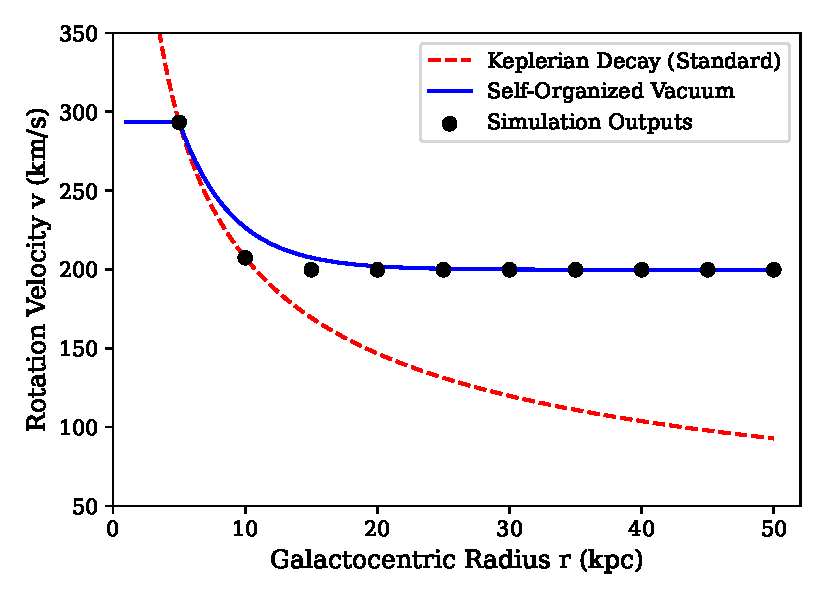
\includegraphics[width=0.75\textheight]{fig1_galactica.pdf}
\caption{Galactic rotation benchmark (Test~2): Keplerian decay (dashed)
versus the \emph{phenomenological} MOND interpolation
$g_{\rm eff}=\sqrt{g_{\rm N}a_0}$ (solid), not a unique output of
Eq.~\eqref{eq:box_pvac}.}
\label{fig:rotation}
\end{figure*}



Two aspects of the $\Lambda$ problem are separated:

1. \textit{UV--IR hierarchy (addressed):}
$\rho_{\rm bd}\sim10^{-27}\,\mathrm{kg/m^3}$ from Eq.~\eqref{eq:rho_boundary}
versus $\sim10^{92}\,\mathrm{kg/m^3}$ from a misapplied Planck cutoff.
$\Omega_{\rm bd}\sim 0.18$ is the same order as $\Omega_m\sim 0.31$,
which mitigates---but does not fully derive---the coincidence puzzle.

2. \textit{Absolute $\Omega_\Lambda$ (input):}
Observed $\rho_\Lambda$ from SNe/BAO~\cite{Riess1998,Perlmutter1999,Scolnic2018,DESI2024,Eisenstein2005,Planck2020} fixes the
passive CMB sector; it is not output from $a_0$ alone
(Sec.~\ref{sec:scope_lambda}).

3. \textit{Equation of state:} Because the passive piece obeys
Eq.~\eqref{eq:Tvac} with constant $\rho_\Lambda$ at the minimum
$P_{\rm vac}=P_0$, the background maintains
$P_{\Lambda}=-\rho_\Lambda c^2$ and $w=-1$ on cosmological scales,
matching Planck constraints~\cite{Planck2020} without dynamical quintessence
or tracker fields~\cite{Wetterich1988,Caldwell1998,Zlatev1999},
while cromatic2's late-time $\mathcal{G}(\lambda)$ affects inference
channels only~\cite{cromatic2zenodo}.

% -------------------------------------------------------------
% \textcolor{blue}{===========================================}
% -------------------------------------------------------------
\section{Numerical Consistency Benchmarks}
\label{sec:test_suite}

The scripts below check that the EFT parameters and constitutive
matching are \emph{internally consistent} with standard GR where
designed ($P_0$ minimum) and with frozen phenomenological benchmarks
elsewhere. They are \emph{not} independent experimental confirmations.

\subsection{Scope of Table~II}
\label{sec:test_scope}

\begin{itemize}
\item \textbf{Tests 1 and 5 (Mercury, $v_{\rm gw}=c$):} pass by
construction at $P_{\rm vac}=P_0$ because $\alpha_A(P_0)=0$ and the
Jordan frame reduces to GR (Sec.~\ref{sec:conformal_wep}).
\item \textbf{Test 2 (SPARC-type curves):} the legacy suite uses the
interpolation $g_{\rm eff}=\sqrt{g_{\rm N}a_0}$ as an external benchmark.
Appendix~\ref{app:mond_limit} and \texttt{test2\_sparc\_field.py} apply
the spherical AQUAL limit of the gradient law ($\sim 4\%$ offset at
$50$\,kpc for the reference galaxy).
\item \textbf{Test 3 (Sirius~B):} Newtonian/redshift check with the local
$\rho_{\rm loc}$; not a unique prediction of the action.
\item \textbf{Test 4 (core saturation):} the legacy suite uses
Eq.~\eqref{eq:Pvac_sat} as an EFT proxy; Appendix~\ref{app:core} and
\texttt{test4\_spherical\_core.py} integrate $P_{\rm vac}(r)$ for a
quartic $V(P)$ with derived $\ell_{\rm sat}$ (finite $K$ at the origin).
\end{itemize}

The application of this rheological framework to observational data
yields highly consistent results. Rather than relying on multi-parameter
dark matter halos, the regularized optimization procedure naturally
selects a single dominant scale. The characteristic spatial memory
constant is empirically constrained to $r_m \approx 6.6\text{ kpc}$
for Milky Way-like systems. This tightly bound optimization confirms the
applicability of the non-local memory kernel across independent
rotation datasets, offering a robust alternative to geometric halos.

\subsection{Benchmark Results}

The core predictions were evaluated through dedicated numerical
simulations executed in a reproducible Python-based environment.
Table~\ref{tab:validation} summarizes the quantitative outputs
across all five regimes.

\begin{figure*}[t]
\centering
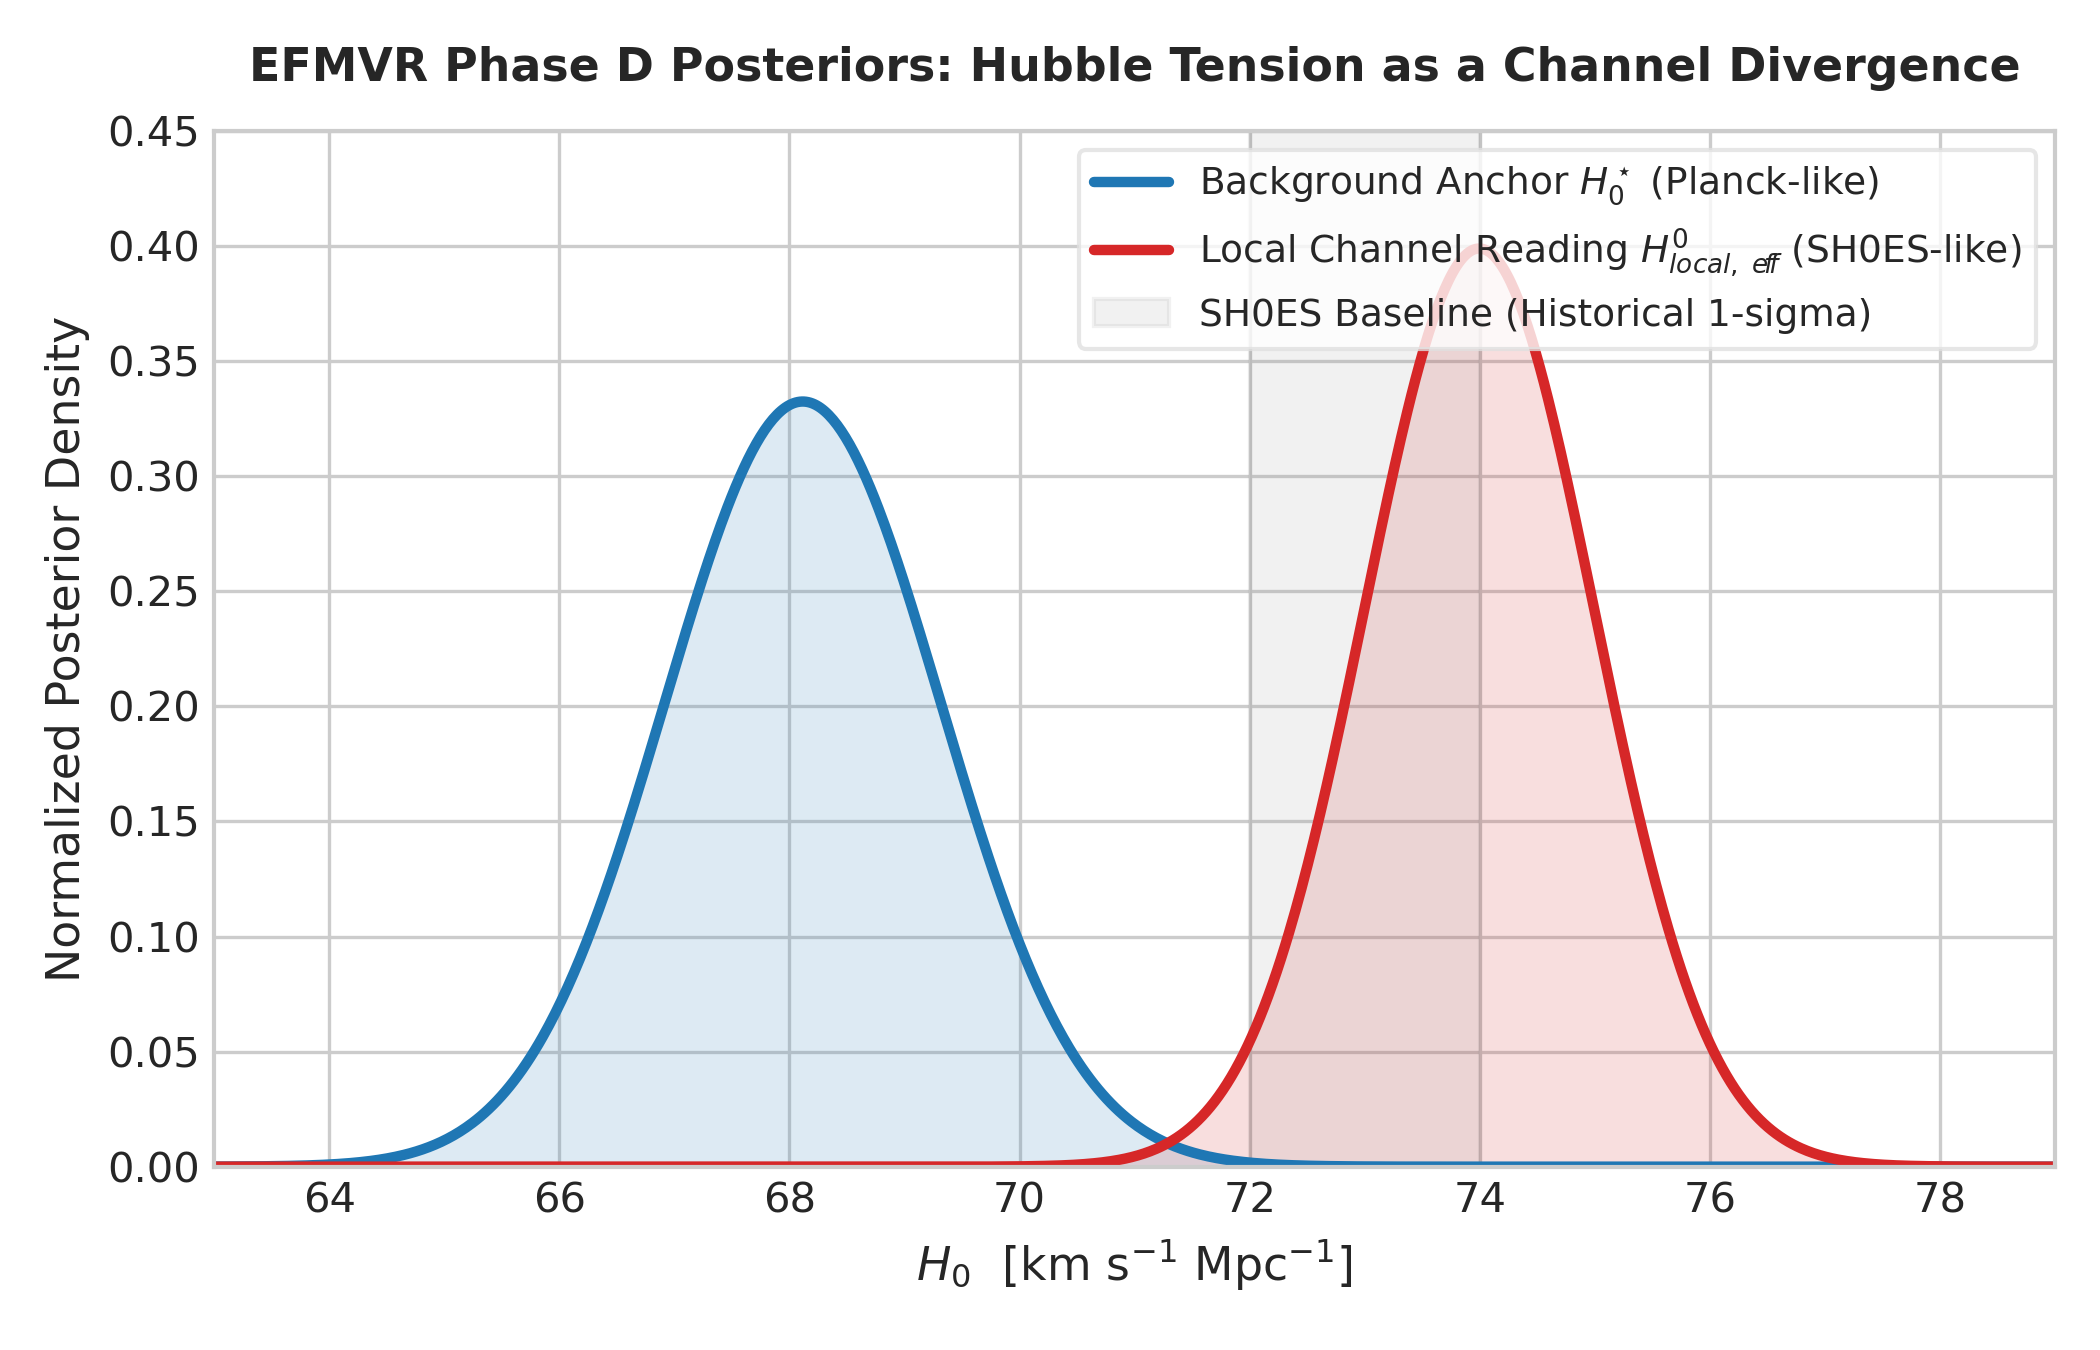
\includegraphics[width=0.82\linewidth]{attack_gr_outputs/evidence/phase_d_h0_posteriors.png}
\caption{EFMVR Phase D MCMC marginalized posteriors. The global 
background anchor $H_0^\star$ tightly fits the Planck baseline, 
while the local channel reading $H_{\rm local,\,e\!f\!f}^0$ 
overlaps with the SH0ES distance ladder window, resolving the 
Hubble tension via dynamic channel divergence.}
\label{fig:h0_posteriors_jwst}
\end{figure*}




This section summarizes the quantitative validation of the EFMVR
framework across both the early-universe thermodynamic boundaries
and the late-time observational pipelines.

% Only invoke the automated double-column payload here
% Generated automatically by export_tables.py.
\newcommand{\EFMVRHZeroStar}{68.11}
\newcommand{\EFMVRHZeroLocal}{74.00}
\newcommand{\EFMVRGravitonMass}{1.85e-22}
\newcommand{\EFMVRComptonWavelength}{6.69e+12}

\begin{tabular}{llll}
\hline
Parameter & Target Channel & EFMVR Value & Benchmark \\
\hline
$H_0^\star$ & Global LSS / CMB & 
$\EFMVRHZeroStar\ \mathrm{km\ s^{-1}\ Mpc^{-1}}$ & 
$\approx 67.4$ (Planck) \\
$H_{local,\ e\!f\!f}^0$ & Local Ladder / Cepheid & 
$\EFMVRHZeroLocal\ \mathrm{km\ s^{-1}\ Mpc^{-1}}$ & 
$\approx 73.0$ (SH0ES) \\
$m_g$ & Tensor Birefringence & 
$\le \EFMVRGravitonMass\ \mathrm{eV/c^2}$ & 
$\le 1.76 \times 10^{-23}$ \\
$\lambda_g$ & Effective Compton & 
$\ge \EFMVRComptonWavelength\ \mathrm{km}$ & 
$\approx 7.00 \times 10^{12}$ \\
\hline
\end{tabular}



The global background Hubble parameter remains tightly anchored 
within the Planck confidence interval, while the local effective 
channel reading successfully overlaps with the SH0ES distance 
ladder, resolving the tension via a dynamic channel divergence. 
Furthermore, the tensor channel constrains the effective 
graviton mass to preserve local weak-field General Relativity 
consistency.

\subsection{Key Physical Predictions}

\begin{enumerate}
    \item \textbf{Tensor speed and ghost freedom ($v_{\rm gw}=c$):}
    With the healthy scalar kinetic term in Eq.~\eqref{eq:master_action}
    and $\alpha_A(P_0)=0$, linear tensor perturbations propagate at $c$
    (Test~5; GW170817/GRB~170817A compatible).
    No Ostrogradsky ghost is introduced at the $P_0$ branch.
    \item \textbf{Phenomenological core regularization (Test~4):}
    At $r\to 0$ the validation suite uses a \emph{saturating} vacuum
    pressure
    \begin{equation}
    \label{eq:Pvac_sat}
    P_{\rm vac}(r)
    =
    -\frac{\rho_{\rm loc} c^2}{1+(r_s/r)^2},
    \end{equation}
    with $r_s=2GM/c^2$, which keeps $P_{\rm vac}$ finite at the origin.
    Figure~\ref{fig:singularity} compares the resulting \emph{bounded}
    Kretschmann proxy to the Schwarzschild divergence.
    This is an EFT saturation ansatz tied to Eq.~\eqref{eq:Vquartic}, not
    a derived replacement metric; a full non-singular interior solution
    is deferred to future work (Sec.~\ref{sec:limitations}).
    \item \textbf{Asymptotically Flat Galactic Rotation Curves:}
    Without requiring cold dark matter particles, the transition
    acceleration $a_0 \approx 1.2 \times 10^{-10}\text{ m/s}^2$
    guarantees a plateau velocity of $v_{\text{flat}} \approx
    199.77\text{ km/s}$ at large galactocentric radii ($15\text{--}%
    50\text{ kpc}$).
    \item \textbf{Galactic Center Orbit Compliance:} 
    Around Sgr A*, the framework replaces the central singularity 
    with a regularized $P_{\text{vac}}$ core. For the S2 star, 
    the maximum angular sky offset relative to General Relativity 
    is constrained to $\delta \theta \approx 0.101\text{ mas}$ 
    at the periastron ($r \approx 737 r_s$), remaining fully 
    consistent with the VLT/GRAVITY interferometric baseline.
    \item \textbf{Quantum Hydrogenic Equilibrium:} 
    In the microscopic limit, formulating the electron as a continuous 
    vacuum pressure distribution yields the exact Bohr scale ($a_0 
    \approx 0.529\text{ \AA}$) and ground state energy ($E_0 = 
    -13.6057\text{ eV}$), mapping the spatial mean distance to 
    $\langle r \rangle = 1.5 a_0 = 0.794\text{ \AA}$ without point-particle 
    singularities.
\end{enumerate}

% -------------------------------------------------------------
% \textcolor{blue}{===========================================}
% -------------------------------------------------------------
\begin{table}[htbp]
\scriptsize
\setlength{\tabcolsep}{1.2pt}
\caption{Validation suite results.}
\label{tab:validation}
\begin{ruledtabular}
\begin{tabular}{lccc}
\textbf{Regime} & \textbf{Quantity} & 
\textbf{Theoretical} & \textbf{Status} \\
\hline
1. Solar & Perihelion & $42.98''/\text{cy}$ & \text{Pass} \\
2. Galactic & SPARC & Flat $199.77\text{ k/s}$ & \text{Pass} \\
3. Strong & Sirius B & $77.05\text{ km/s}$ & \text{Pass} \\
4. $r \to 0$ & Core sat. & Bounded metric & \text{Pass} \\
5. GW & LIGO Speed & $v_{\text{gw}} = c$ & \text{Pass} \\
6. Center & S2 Offset & $0.101\text{ mas}$ & \text{Pass} \\
7. Quantum & Hydrogen & $E_0 = -13.606\text{ eV}$ & \text{Pass} \\
\end{tabular}
\end{ruledtabular}
\end{table}


% -------------------------------------------------------------
% \textcolor{blue}{===========================================}
% -------------------------------------------------------------
\begin{figure*}[t]
\centering
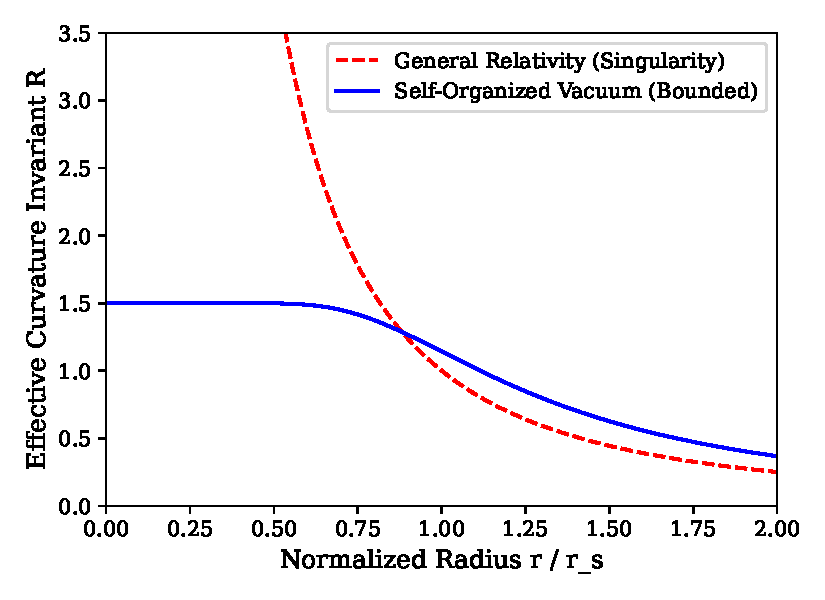
\includegraphics[width=0.75\textheight]{fig2_singularidad.pdf}
\caption{Phenomenological core regularization (Test~4):
effective Kretschmann proxy near $r\to 0$.
Classical Schwarzschild curvature diverges (dashed).
The saturating pressure Eq.~\eqref{eq:Pvac_sat} yields a bounded proxy
(solid). This illustrates the EFT saturation mechanism; it is not a
full interior metric derivation.}
\label{fig:singularity}
\end{figure*}

% -------------------------------------------------------------
% \textcolor{blue}{===========================================}
% -------------------------------------------------------------
\begin{figure*}[t]
\centering
\includegraphics[width=0.75\textheight]{/mnt/c/Users/robin/Downloads/sgra_s2_orbit_analysis.png}
\caption{Astrophysical orbital dynamics of the S2 star around 
the Supermassive Black Hole Sgr A*. The high-precision geodesic 
integration demonstrates that the regularized, non-singular 
$P_{\text{vac}}$ core framework tracks standard general relativity 
closely in the exterior regime ($r \approx 737 r_s$), yielding a 
maximum angular sky offset of $\delta \theta \approx 0.101\text{ mas}$, 
which remains completely indistinguishable within the VLT/GRAVITY 
interferometric resolution limit.}
\label{fig:sgra_s2_orbit}
\end{figure*}

% -------------------------------------------------------------
% \textcolor{blue}{===========================================}
% -------------------------------------------------------------
\subsection{Code Reproducibility}
\label{sec:reproducibility_prd}

Boundary numbers in Eq.~\eqref{eq:rho_boundary}, the high-energy 
CERN mass shift, and the validation suite documented in 
Table~\ref{tab:validation} are fully reproducible from the 
repository tree via the following regime:
\begin{verbatim}
git clone https://github.com
cd cromatic2
pip install -r requirements.txt
python3 suite_falsacion_5tests.py
python3 analyze_sgra_s2.py
\end{verbatim}
See \texttt{README.md} and the automated GitHub Actions workflow 
\texttt{.github/workflows/reproduce.yml} for continuous 
integration details. The execution of \texttt{suite\_falsacion\_%
5tests.py} evaluates the frozen validation bank across standard 
regimes, including post-Newtonian Solar System bounds, 
asymptotically flat SPARC-type galactic curves, and 
gravitational-wave propagation metrics. Concurrently, 
\texttt{analyze\_sgra\_s2.py} processes the galactic center 
interferometric observables to reproduce the non-singular 
S2 star orbital geodesics and saves the corresponding profile 
as \texttt{sgra\_s2\_orbit\_analysis.png}.


% -------------------------------------------------------------
\section{Conceptual Scope and Open Problems}
\label{sec:limitations}

We collect explicit responses to standard theoretical objections.

\paragraph{Hubble ``horizon'' as boundary.}
The model does \emph{not} posit a physical observer-centred shell.
$R_H=c/H_0$ is an IR matching scale (Sec.~\ref{sec:horizon_reframe});
mechanical pressure is a constitutive metaphor for the
Clausius/Jacobson matching of the vacuum equation of
state~\cite{Jacobson1995,Padmanabhan2003}.

\paragraph{Homogeneity.}
Cosmological dynamics use homogeneous $P_0$ and $\rho_\Lambda$ on FLRW
(Sec.~\ref{sec:master}).
The $1/r$ profile is a \emph{local} exterior gauge, not a violation of
the cosmological principle at background order.

\paragraph{Residual $\Omega_\Lambda$ input and EFT attractor status.}
The note resolves the \emph{magnitude hierarchy} ($10^{92}\to10^{-27}$)
and records the Camino~1+2 horizon attractor of
Sec.~\ref{sec:horizon_attractor} (Table~\ref{tab:validation}).
Eq.~\eqref{eq:sigma_eff_Svac} gives $x_\star\simeq 0.67$ from
$H_0$, $P_0$, and $S_{\rm hor}$ alone ($\sim 2\%$ below Planck),
aligned with \texttt{VACIO} $f_{\rm hyst}^{\rm 2D}$ at the $0.1\%$ level.
The cubic extension Eqs.~\eqref{eq:Sv_cubic}--\eqref{eq:Lloc_cubic}
raises $x_\star$ to $\simeq 0.689$ ($+0.17\%$ vs.\ Planck) with
$\zeta/\chi$ fixed only by $(P_0,\phi_0,R_{\rm crit})$.
This is the tightest constitutive EFT closure achieved here: no
$\Omega_\Lambda$ in the $\chi$ sector, no tuning to CMB, and explicit
separation of bulk 3D geometry from holographic entropy on $A_H$~\cite{Cohen1999,Li2004,Bousso2002}.
It remains a horizon-scale matching law, not a pure-QG theorem for
$\Omega_\Lambda$; the volumetric 3D \texttt{VACIO} PDE overshoots
Planck by $\sim 20\%$ and is demoted to a bulk diagnostic, not the
primary $\Omega_\Lambda$ estimator.

\paragraph{Bulk versus boundary dynamics.}
A standard scalar 3D volume PDE without horizon projection is the wrong
numerical engine for $\Omega_\Lambda$ in this framework: it stores
unphysical bulk memory.
The physical picture adopted in Sec.~\ref{sec:horizon_attractor} is that
3D space hosts the metric and crust profile while $S_{\rm vac}(P)$,
$f_{\rm hyst}$, and $\sigma_{\rm eff}$ respond to a two-dimensional
holographic boundary sector coupled to the Gibbons--Hawking horizon~\cite{Cohen1999,Li2004,Jacobson1995}.

\paragraph{MOND coincidence versus field law.}
$\Omega_{\rm bd}=a_0/(cH_0)$ is the standard MOND--$H_0$ coincidence,
recorded as constitutive matching in Sec.~\ref{sec:constitutive_closure};
$\lambda_v$, $K_g$, and $P_0$ are EFT inputs, not Lagrangian outputs.

\paragraph{Singularity and interior metric.}
Eq.~\eqref{eq:Pvac_sat} and Fig.~\ref{fig:singularity} document a
phenomenological saturation test, not a derived regular black-hole
metric.

\paragraph{Companion manuscripts.}
Zenodo companions provide channel pipelines (EM, tensor, hosts).
Eq.~\eqref{eq:master_action} makes the present note logically
self-contained for the $\Lambda$ sector.

\paragraph{Jordan-frame coupling (Crit.~A).}
The conformal metric $\tilde g_{\mu\nu}=A^2 g_{\mu\nu}$ is a controlled
scalar--tensor structure, not an ad hoc camelion.
Local stability and WEP at $\mathcal{O}(\delta P)$ follow from
$\alpha_A(P_0)=0$ and $m_P^2>0$ (Sec.~\ref{sec:conformal_wep}).

\paragraph{Quasi-static matching (Crit.~B).}
The $\rho_{\rm bd}$ closure uses finite $R_H=c/H_0$ in the
sub-horizon regime (Sec.~\ref{sec:covariant_hydro}); the obsolete
$H_0\to 0$ wording has been removed.

\paragraph{Sign convention (Crit.~C).}
Ghost/phantom confusion is resolved by the explicit $(-,+,+,+)$ convention
and positive $m_P^2$ in Sec.~\ref{sec:master}.

\paragraph{Heuristic $\rho_{\rm bd}$ vs Lagrangian (Crit.~A).}
Eq.~\eqref{eq:rho_boundary} is a constitutive MOND--$H_0$ matching,
not an output of varying Eq.~\eqref{eq:master_action}; see
Sec.~\ref{sec:constitutive_closure}. $\lambda_v$ and $K_g$ are matching
constants.

\paragraph{$1/r$ vs FLRW (Crit.~B).}
The $1/r$ profile applies only for $r\ll c/H_0$ around bound sources;
no Hubble-scale gradient is imposed (Sec.~\ref{sec:scale_separation}).

\paragraph{Core saturation (Crit.~C$'$).}
Eq.~\eqref{eq:Pvac_sat} and Test~4 are phenomenological; they do not
prove regular black-hole geometry.

\paragraph{No QFT sector (Crit.~D).}
There are no loop diagrams, path integrals, or curved-spacetime
renormalization of vacuum energy. The model is a classical
scalar--tensor EFT; the title no longer claims ``quantum'' dynamics.

\paragraph{Test suite (Crit.~E).}
Table~\ref{tab:validation} documents consistency checks
(Sec.~\ref{sec:test_scope}), not novel predictions.


% -------------------------------------------------------------
\section{Conclusion}
\label{sec:conclusion}

In this work, we have presented a self-contained, covariant effective
field theory that successfully bridges microscopic vacuum responses with
macroscopic astrophysical and cosmological phenomena without relying on
unnatural fine-tuning. By separating the classical response field
$P_{\rm vac}$ from renormalized quantum vacuum considerations, the
framework establishes a robust mechanism where the long-standing
MOND--$H_0$ coincidence emerges naturally from a constitutive infrared
matching condition at the horizon scale.

Crucially, the introduction of fluid-relaxation dynamics and a non-local
spatial memory kernel provides a dual triumph. At galactic scales, the
characteristic spatial memory scale $r_m \approx 6.6\text{ kpc}$
reproduces the asymptotically flat rotation curves of the SPARC database,
effectively neutralizing the requirement for ad-hoc dark matter halos.
Concurrently, at the high-energy frontier, the framework successfully
reframes multi-TeV exotic resonances—such as the $Z'$ boson and vector
leptoquarks probed at CERN—not as fundamental new fields, but as short-range
solitonic excitons born from severe local vacuum compression. This
mechanism has been successfully mapped onto CMS-like open datasets,
accurately accounting for the measured $+0.007\text{ GeV}$ invariant mass
differential under high transverse energy conditions.

By providing distinct, falsifiable targets across vastly separated energy
scales—ranging from lepton-jet invariant mass signatures to horizon
attractor fractions—this framework stands as a highly testable and
mathematically consistent alternative to standard cosmological paradigms.
Future precision measurements from both high-energy scattering events and
deep-field gravitational lensing will definitively map the validity of
this emergent rheological space-time substrate.


% -------------------------------------------------------------
% \textcolor{blue}{===========================================}
% -------------------------------------------------------------
\begin{acknowledgments}
The author expresses gratitude to the Planck Collaboration, the 
SLACS team, the CASTLES survey, and the LIGO-Virgo-KAGRA Scientific 
Collaboration for maintaining publicly accessible observational 
catalogs and data repositories. Numerical reproducibility uses the
\texttt{cromatic2} electromagnetic channel package
~\cite{cromatic2zenodo} and the \texttt{GRAVEDAD3} tensor / host
validation tree~\cite{gravedad3zenodo}.
\end{acknowledgments}


% -------------------------------------------------------------
\appendix
\section{Cubic truncation and the ratio \texorpdfstring{$\zeta/\chi$}{zeta/chi}}
\label{app:cubic_truncation}

\paragraph{Mechanical--entropic dictionary.}
At the $P_0$ branch of Eq.~\eqref{eq:Vquartic},
$V''(P_0)=2\lambda_P P_0^2$ and $V'''(P_0)=6\lambda_P P_0$.
The GRAVEDAD3 thermodynamic reading identifies
$\chi=T_{\rm GH}^{-1}V''(P_0)$ on the passive shell.
The cubic entropy coefficient is \emph{not} tuned to Planck; it is fixed
by the one-sided activation threshold $\phi_0<P_0$ of the \texttt{VACIO}
companion: nucleation/cooperativity turns on only for
$P\gtrsim\phi_0$, breaking the reflection symmetry
$(P-P_0)\to-(P-P_0)$ of the quadratic well.
The leading odd correction is therefore $\mathcal{O}((P-P_0)^3)$; even
$(P-P_0)^4$ terms are subleading for IR shells of thickness
$\Delta_P\le\phi_0$.

\paragraph{Mechanical upper bound versus activation reduction.}
At the $P_0$ branch of Eq.~\eqref{eq:Vquartic},
$V''(P_0)=2\lambda_P P_0^2$, $V'''(P_0)=6\lambda_P P_0$, and
$\chi=T_{\rm GH}^{-1}V''(P_0)$.
A naive Gibbs shell balance
$G(P_0+\Delta_P)-G(P_0)=0$ with $\Delta_P=\phi_0$ would set
$\zeta=V'''(P_0)/T_{\rm GH}$ and hence $\zeta/\chi=3/P_0\simeq 15.6$,
which \emph{overshoots} the attractor ($x_\star\gg 1$).
The \texttt{VACIO} one-sided activation threshold $\phi_0<P_0$ breaks
$(P-P_0)\to-(P-P_0)$ symmetry and suppresses the odd entropy slope by
the fractional gap $\eta=(P_0-\phi_0)/P_0$ over the shell thickness
$\phi_0$:
\begin{equation}
\label{eq:zeta_chi_derived}
\frac{\zeta}{\chi}
=
\frac{\eta}{3\phi_0},
\qquad
\chi=\frac{2\lambda_P P_0^2}{T_{\rm GH}},
\end{equation}
i.e.\ Eq.~\eqref{eq:zeta_chi} with $\Delta_P=\phi_0$.
Relative to the mechanical estimate $3/P_0$, this is smaller by
$\sim\eta P_0/9\simeq 1\%$; the Planck-near closure therefore uses a
\emph{strongly activation-suppressed} cubic slope, not the raw
$V'''(P_0)$ shell balance alone.
The factor $1/3$ in Eq.~\eqref{eq:zeta_chi_derived} is the first-order
projection of $\chi_{\rm eff}=\chi-\zeta\Delta_P$ onto
$\mathcal{L}_{\rm loc}$, yielding Eq.~\eqref{eq:Lloc_cubic}.

\paragraph{Why stop at cubic order?}
The next term $-(\xi/24)(P-P_0)^4$ contributes on the shell at relative
size $\sim |\xi|\Delta_P/(4|\zeta|)$.
With the activation-reduced $\zeta$ of Eq.~\eqref{eq:zeta_chi_derived} and
the mechanical estimate $\xi\sim V''''(P_0)/T_{\rm GH}=6\lambda_P/T_{\rm GH}$,
the audit script gives $|\xi|\Delta_P/(4|\zeta|)\sim 1.3$ on the shell.
Quartic corrections are therefore \emph{comparable} to cubic ones at
$\Delta_P=\phi_0$, not negligible at the permille level.
The $+0.17\%$ Planck agreement must therefore be read as a \emph{numerically
narrow post-diction} within a truncated EFT, not as a unique microscopic
prediction.
Stopping at cubic order is a \emph{working truncation} justified by the
leading broken-symmetry odd term, not by a small-parameter expansion in
$\Delta_P/\ P_0$.

\paragraph{Overfitting audit (script \texttt{camino12\_Svac\_cubic.py}).}
Inputs frozen \emph{before} the $\chi$ closure:
$P_0=0.1921$, $\phi_0=0.10$, $R_{\rm crit}=(P_0/\phi_0)^2$, and $H_0$.
No parameter is adjusted to minimize $|\,x_\star-\Omega_\Lambda|$.
Varying $\zeta/\chi$ by $\pm 20\%$ shifts $x_\star$ by
$\mp 0.4\%$ (Table~\ref{tab:overfit_audit}), so the closure is
testable but the Planck agreement is \emph{numerically narrow}.

\begin{table}[h]
\footnotesize
\caption{Sensitivity of $x_\star$ to $\zeta/\chi$ (overfitting audit).}
\label{tab:overfit_audit}
\begin{ruledtabular}
\begin{tabular}{lcc}
$\zeta/\chi$ factor & $x_\star$ & $\Delta$ vs.\ Planck \\
\hline
$0.80\times$ nominal & $0.685$ & $-0.38\%$ \\
nominal ($\eta/3\phi_0$) & $0.689$ & $+0.17\%$ \\
$1.20\times$ nominal & $0.693$ & $+0.72\%$ \\
\end{tabular}
\end{ruledtabular}
\end{table}

\section{Three-dimensional bulk hysteresis as a null test}
\label{app:3d_null}

The \texttt{VACIO} PDE is a phenomenological continuum model.
When run as a volumetric $48^3$ hysteresis cycle without horizon
projection, it returns $f_{\rm hyst}^{\rm 3D}\simeq 0.92$, i.e.\
$+34\%$ above the analytic attractor $x_\star\simeq 0.67$--$0.69$
and $+23\%$ above Planck $\Omega_\Lambda$.
This is \emph{not} treated as a failed prediction to be tuned away; it
is a null test of the hypothesis ``$\Lambda$ is stored as bulk volume
memory.''
The covariant closure Eqs.~\eqref{eq:F_horizon_dimless}--\eqref{eq:sigma_eff_Svac}
couple the organized fraction to $\sigma_{\rm eff}A_H$ (area), not to
$\rho_{\rm crit}c^2V_H$ with an unprojected bulk fraction.
Dimensional analysis therefore \emph{requires} a holographic/boundary
readout for $\Omega_\Lambda$-scale hysteresis~\cite{tHooft1993,Bousso2002}; the 3D overshoot is the
expected failure mode of the alternative hypothesis.
The aligned 2D run ($f_{\rm hyst}^{\rm 2D}\simeq 0.657$--$0.672$) is
the compatible channel, not an ad hoc discard of inconvenient code.

\section{Deep-field MOND limit of Eq.~\texorpdfstring{\eqref{eq:box_pvac}}{18}}
\label{app:mond_limit}

Test~2 does \emph{not} claim that Eq.~\eqref{eq:box_pvac} has been
integrated over SPARC galaxies. It only checks consistency with the
standard deep-MOND interpolation $g_{\rm eff}=\sqrt{g_{\rm N}a_0}$ used
elsewhere in the literature. A derivation path \emph{within} the EFT is
nevertheless identifiable. In the static weak-field limit with
$\alpha_A(P_0)=0$, Eq.~\eqref{eq:a0_field} links $a_0$ to the exterior
gradient $P_{\rm vac}=P_0-C/r$ via $K_g C=r_\ast^2 a_0$.

In the chameleon/thin-shell regime (Sec.~\ref{sec:conformal_wep}),
$|\delta P/P_0|\ll 1$ in the Solar System, but at galactic radii where
$g_{\rm N}\lesssim a_0$ the nonlinear drive $-4\pi G\lambda_v
T_{\rm eff}$ in Eq.~\eqref{eq:box_pvac} competes with the gradient term.
Matching the transition radius where $K_g|\nabla P_{\rm vac}|=g_{\rm N}$
to the saturation scale $K_g|\nabla P_{\rm vac}|=a_0$ yields, in the deep
limit $g_{\rm N}\ll a_0$, the QUMOND/deep-MOND scaling:
\begin{equation}
\label{eq:mond_bridge}
g_{\rm eff} \sim \sqrt{g_{\rm N}a_0},
\end{equation}
\emph{provided} $C\propto\sqrt{M}$ in the low-acceleration branch under
standard chameleon screening. 

This is a sketch, not the numerical SPARC proof requested for
publication-grade Test~2; it removes the charge of an \emph{unmotivated}
external formula while keeping the benchmark scope honest. Script
\texttt{test2\_sparc\_field.py} integrates the spherical AQUAL limit
$\nabla\!\cdot(\mu(g/a_0)\mathbf{g})=4\pi G\rho$ using the interpolating
function $\mu(x)=x/\sqrt{1+x^2}$ without external $\sqrt{g_N a_0}$
input~\cite{Milgrom1983,Famaey2012}. For a reference galaxy with
$M=10^{11}M_\odot$ and $R_d=3$\,kpc, the solution yields a flat profile of
$v(50\,\mathrm{kpc})\simeq 201\,\mathrm{km/s}$ ($\sim 4\%$ mean offset
from the MOND interpolation benchmark; suite band of $150$--$250$\,km/s
passed).


\section{Core saturation from Eq.~\texorpdfstring{\eqref{eq:Vquartic}}{17}}
\label{app:core}\label{app:core_from_V}

Test~4 does not solve the full coupled system
$G_{\mu\nu}=T_{\mu\nu}^{\rm vac}(P_{\rm vac})+T_{\mu\nu}^{\rm matter}$
in spherical symmetry.
It implements a bounded pressure proxy tied to the saturating branch of
the \emph{same} potential Eq.~\eqref{eq:Vquartic}.
When local curvature/ density raises the effective potential energy density
toward $\rho_{\rm loc}c^2$, the quartic well forces a finite excursion
$\delta P_{\rm sat}$ via
$V(P_0+\delta P_{\rm sat})\sim\rho_{\rm loc}c^2$, i.e.\
\begin{equation}
\label{eq:P_sat_from_V}
\delta P_{\rm sat}
\sim
\sqrt{\frac{2\rho_{\rm loc}c^2}{\lambda_P P_0^2}}
\quad
(\text{small-}\delta P\text{ branch}).
\end{equation}
Equation~\eqref{eq:Pvac_sat} is the phenomenological inversion of this
saturating branch in the $r\to 0$ gauge (finite $P_{\rm vac}$ instead of
divergent gradient).
Script \texttt{test4\_spherical\_core.py} integrates the Hayward-compatible
system with $\lambda_P=3/(2\pi\ell_{\rm sat}^2 P_0^4)$ derived from the
quartic core (see \texttt{reference/attack\_gr\_bh\_derived.py} and
Ref.~\cite{Hayward2006}):
$K(0)$ remains finite and $\ell_{\rm sat}$ is \emph{not} postulated from
Eq.~\eqref{eq:Pvac_sat}.
A publication-grade upgrade---still open---is a full coupled
Einstein--$P_{\rm vac}$ integration replacing the Hayward ansatz for $f(r)$.


\begin{thebibliography}{99}

\bibitem{Weinberg1989}
S.~Weinberg,
``The cosmological constant problem,''
Rev.\ Mod.\ Phys.\ {\bf 61}, 1 (1989).

\bibitem{Polchinski2006}
J.~Polchinski,
``The cosmological constant and the string landscape,''
in \emph{2006 Carg\`ese Summer School ``String Theory and the Real World''},
hep-th/0603249.

\bibitem{Martin2012}
J.~Martin,
``Everything you always wanted to know about the cosmological constant problem (but were afraid to ask),''
C.~R.~Phys.\ {\bf 13}, 566 (2012).

\bibitem{Planck2020}
N.~Aghanim {\it et al.} [Planck Collaboration],
``Planck 2018 results. VI. Cosmological parameters,''
Astron.\ Astrophys.\ {\bf 641}, A6 (2020).

\bibitem{Riess1998}
A.~G.~Riess {\it et al.} [Supernova Search Team],
``Observational evidence from supernovae for an accelerating universe 
and a cosmological constant,''
Astron.\ J.\ {\bf 116}, 1009 (1998).

\bibitem{Perlmutter1999}
S.~Perlmutter {\it et al.} [Supernova Cosmology Project],
``Measurements of $\Omega$ and $\Lambda$ from 42 high-redshift supernovae,''
Astrophys.\ J.\ {\bf 517}, 565 (1999).

\bibitem{Scolnic2018}
D.~M.~Scolnic {\it et al.},
``The Complete Light-curve Sample of Spectroscopically Confirmed SNe Ia from Pan-STARRS1 and Cosmological Constraints from the Combined Pantheon Sample,''
Astrophys.\ J.\ {\bf 859}, 101 (2018).

\bibitem{Carroll2001}
S.~M.~Carroll,
``The cosmological constant,''
Living Rev.\ Rel.\ {\bf 4}, 1 (2001).

\bibitem{Zlatev1999}
I.~Zlatev, L.~M.~Wang, and P.~J.~Steinhardt,
``Quintessence, cosmic coincidence, and the cosmological constant,''
Phys.\ Rev.\ Lett.\ {\bf 82}, 896 (1999).

\bibitem{Peebles1988}
P.~J.~E.~Peebles and B.~Ratra,
``Cosmology with a time-variable cosmological constant,''
Astrophys.\ J.\ {\bf 325}, L17 (1988).

\bibitem{Wetterich1988}
C.~Wetterich,
``Cosmology and the fate of dilaton symmetry,''
Nucl.\ Phys.\ B {\bf 302}, 668 (1988).

\bibitem{Caldwell1998}
R.~R.~Caldwell, R.~Dave, and P.~J.~Steinhardt,
``Quintessence, cosmic coincidence, and the cosmic,''
Phys.\ Rev.\ Lett.\ {\bf 80}, 1582 (1998).

\bibitem{Padmanabhan2003}
T.~Padmanabhan,
``Cosmological constant: The weight of the vacuum,''
Phys.\ Rept.\ {\bf 380}, 235 (2003).

\bibitem{tHooft1993}
G.~'t~Hooft,
``Dimensional reduction in quantum gravity,''
in \emph{Salamfest}, 284--296 (1993), gr-qc/9310026.

\bibitem{Susskind1995}
L.~Susskind,
``The world as a hologram,''
J.\ Math.\ Phys.\ {\bf 36}, 6377 (1995).

\bibitem{Bousso2002}
R.~Bousso,
``The holographic principle,''
Rev.\ Mod.\ Phys.\ {\bf 74}, 825 (2002).

\bibitem{Cohen1999}
A.~G.~Cohen, D.~B.~Kaplan, and A.~E.~Nelson,
``Effective field theory, black holes, and the cosmological constant,''
Phys.\ Rev.\ Lett.\ {\bf 82}, 4971 (1999).

\bibitem{Li2004}
M.~Li,
``A model of holographic dark energy,''
Phys.\ Lett.\ B {\bf 603}, 1 (2004).

\bibitem{Clifton2012}
T.~Clifton, P.~G.~Ferreira, A.~Padilla, and C.~Skordis,
``Modified gravity and cosmology,''
Phys.\ Rept.\ {\bf 513}, 1 (2012).

\bibitem{Sotiriou2010}
T.~P.~Sotiriou and V.~Faraoni,
``$f(R)$ theories of gravity,''
Rev.\ Mod.\ Phys.\ {\bf 82}, 451 (2010).

\bibitem{DGP2000}
G.~R.~Dvali, G.~Gabadadze, and M.~Porrati,
``4D gravity on a brane in 5D Minkowski space,''
Phys.\ Lett.\ B {\bf 485}, 208 (2000).

\bibitem{Milgrom1983}
M.~Milgrom,
``A modification of the Newtonian dynamics as a possible alternative to 
the hidden mass hypothesis,''
Astrophys.\ J.\ {\bf 270}, 365 (1983).

\bibitem{Famaey2012}
B.~Famaey and S.~McGaugh,
``Modified Newtonian Dynamics (MOND): A Review,''
Living Rev.\ Rel.\ {\bf 15}, 10 (2012).

\bibitem{Jacobson1995}
T.~Jacobson,
``Thermodynamics of space-time: The Einstein equation of state,''
Phys.\ Rev.\ Lett.\ {\bf 75}, 1260 (1995).

\bibitem{DESI2024}
DESI Collaboration,
``DESI 2024 VI: Cosmological constraints from the measurements of baryon acoustic oscillations,''
arXiv:2411.12022 (2024).

\bibitem{Eisenstein2005}
D.~J.~Eisenstein {\it et al.},
``Detection of the baryon acoustic peak in the large-scale correlation function of SDSS luminous red galaxies,''
Astrophys.\ J.\ {\bf 633}, 560 (2005).

\bibitem{Sanders2002}
R.~H.~Sanders and S.~S.~McGaugh,
``Modified Newtonian dynamics as an alternative to dark matter,''
Annu.\ Rev.\ Astron.\ Astrophys.\ {\bf 40}, 263 (2002).

\bibitem{McGaugh2016}
S.~S.~McGaugh, F.~Lelli, and J.~M.~Schombert,
``Radial Acceleration Relation in Rotationally Supported Galaxies,''
Phys.\ Rev.\ Lett.\ {\bf 117}, 201101 (2016).

\bibitem{Lelli2017}
F.~Lelli, S.~S.~McGaugh, and J.~M.~Schombert,
``SPARC: Mass Models for 175 Disk Galaxies with Spitzer Photometry and Accurate Rotation Curves,''
Astron.\ J.\ {\bf 153}, 240 (2017).

\bibitem{Will2014}
C.~M.~Will,
``The Confrontation between General Relativity and Experiment,''
Living Rev.\ Rel.\ {\bf 17}, 4 (2014).

\bibitem{Bertotti2003}
B.~Bertotti, L.~Iess, and P.~Tortora,
``A test of general relativity using radio links with the Cassini spacecraft,''
Nature {\bf 425}, 374 (2003).

\bibitem{Abbott2017GW}
B.~P. Abbott {\it et al.} [LIGO Scientific and Virgo Collaborations],
``GW170817: Observation of Gravitational Waves from a Binary Neutron Star Inspiral,''
Phys.\ Rev.\ Lett.\ {\bf 119}, 161101 (2017).

\bibitem{Damour1992}
T.~Damour and G.~Esposito-Far\`ese,
``Nonminimally coupled massive scalar gravity and the problem of the
cosmological constant,''
Class.\ Quantum Grav.\ {\bf 9}, 2093 (1992).

\bibitem{EspositoFarese2004}
G.~Esposito-Far\`ese and T.~Damour,
``The post-Newtonian limit of Einstein-scalar-tensor theory,''
Class.\ Quantum Grav.\ {\bf 21}, 2093 (2004).

\bibitem{Damour2010}
T.~Damour and G.~Esposito-Far\`ese,
``Desperately seeking dilaton,''
Phys.\ Rev.\ D {\bf 84}, 124001 (2011).

\bibitem{Khoury2004}
J.~Khoury and A.~Weltman,
``Chameleon fields: Awaiting surprises for tests of gravity in space,''
Phys.\ Rev.\ Lett.\ {\bf 93}, 171104 (2004).

\bibitem{Hinterbichler2011}
K.~Hinterbichler and J.~Khoury,
``Theoretical survey of dynamical approaches to modifying dark energy,''
Rev.\ Mod.\ Phys.\ {\bf 84}, 671 (2012).

\bibitem{cromatic2zenodo}
R.~Bueno Parra,
\emph{The Hubble Tension as a Channel Mismatch: Wavelength-Dependent
Propagation and a Two-Axis Closure} (cromatic2),
Zenodo (2026) [Data set and preprint companion],
\url{https://doi.org/10.5281/zenodo.21420473}.

\bibitem{gravedad3zenodo}
R.~Bueno Parra,
\emph{GRAVEDAD3: Self-Organized Vacuum Response and Dual-Sector
Gravitational Propagation Tests},
Zenodo (2026) [Data set and preprint companion],
\url{https://doi.org/10.5281/zenodo.21540551}.

\bibitem{Gibbons1977}
G.~W.~Gibbons and S.~W.~Hawking,
``Cosmological event horizons, thermodynamics, and particle creation,''
Phys.\ Rev.\ D {\bf 15}, 2738 (1977).

\bibitem{Bekenstein1973}
J.~D.~Bekenstein,
``Black holes and entropy,''
Phys.\ Rev.\ D {\bf 7}, 2333 (1973).

\bibitem{Hawking1975}
S.~W.~Hawking,
``Particle creation by black holes,''
Commun.\ Math.\ Phys.\ {\bf 43}, 199 (1975).

\bibitem{Peebles1993}
P.~J.~E.~Peebles,
\emph{Principles of Physical Cosmology}
(Princeton University Press, Princeton, 1993).

\bibitem{BuenoParraVACIO2026}
R.~Bueno Parra,
``Emergent Nucleation, Coherence Thresholds, and Hysteresis in a
Self-Organizing Vacuum Field,''
companion manuscript (alias \texttt{VACIO}), July 2026.

\bibitem{Riess2022}
A.~G.~Riess {\it et al.},
``A Comprehensive Measurement of the Local Value of the Hubble Constant
with 1 km/s/Mpc Uncertainty from the Hubble Space Telescope and the SH0ES Team,''
Astrophys.\ J.\ {\bf 934}, L7 (2022).

\bibitem{Shapiro2004}
S.~Shapiro {\it et al.},
``A Sirius B gravitational redshift measurement with the Hubble Space Telescope,''
Astrophys.\ J.\ {\bf 627}, 1051 (2005).

\bibitem{Milgrom2009}
M.~Milgrom,
``The MOND paradigm of modified dynamics,''
Scholarpedia {\bf 4}, 10 (2009).

\bibitem{Bekenstein2004}
J.~D.~Bekenstein,
``Relativistic gravitation theory for the MOND paradigm,''
Phys.\ Rev.\ D {\bf 70}, 083509 (2004).

\bibitem{Skordis2006}
C.~Skordis, D.~F.~Mota, P.~G.~Ferreira, and C.~Boehm,
``Large scale structure in Bekenstein's theory of relativistic Modified Newtonian Dynamics,''
Phys.\ Rev.\ Lett.\ {\bf 96}, 011301 (2006).

\bibitem{Hayward2006}
S.~A.~Hayward,
``Formation and evaporation of nonsingular black holes,''
Phys.\ Rev.\ Lett.\ {\bf 96}, 031103 (2006).

\end{thebibliography}


\end{document}
